\section{The stochastic automaton on each shell}\label{sec:ca}
\stagebox{\statusbuilt}{\src{core/src/ca.rs}}

The automaton makes the discrete decisions about a bud: how many petals it
has, where each one attaches, how tall it may grow, and which patch of its
shell it ends up owning. It is a cellular automaton with stochastic rules
(strictly not a pure CA, because a cell's update draws random numbers and
initiation reads a non-local field). It runs once per flower, from the
flower's traits and stream 1 of the flower's seed (\cref{sec:seeds}), so
siblings get different petal counts and placements from the same rules.

This section first states the rules exactly, then explains what each one does
to the result, and then follows one real flower through every step
(\cref{sec:ca-example}).

\subsection{Inputs and outputs}
\paragraph{Inputs.} From the flower's traits (\cref{sec:traits}): the layer
count $L$, the inhibition reach $\sigma$ and threshold $\tau$, the initiation
probability $p_{\mathrm{init}}$, the stagger weight $\beta$, the claim
probabilities $p_\uparrow$ and $p_\leftrightarrow$, and the inner height
fraction $h_{\mathrm{in}}$. From the shells (\cref{sec:shells}): the scaled
radius $a_k$ of each layer's mid-surface, which sets how long an arc of the
shell is. Nothing else: the automaton does not see thicknesses, growth traits
or the sepals.

\paragraph{Output.} One grid of owners per layer, and for each petal its
layer, base angle, height cap and per-row shape (\cref{sec:ca-output}).

\subsection{The grid}\label{sec:ca-grid}
Each shell carries a grid of $\NA = 96$ azimuth cells by $\NP = 28$ polar
rows, stored row by row. Cell $(r,s)$ has azimuth
\[
  \theta_s = \Bigl(s + \tfrac12\Bigr)\frac{2\pi}{\NA}, \qquad s = 0,\dots,\NA-1,
\]
so one cell is $3.75^\circ$ wide, and the grid wraps around in $s$: cell
$\NA-1$ is the left neighbour of cell 0. Row 0 is the attachment ring at the
bottom of the shell and rows run upward. When the sheet stage later places a
row on the shell, row $r$ sits at polar angle
\[
  \phi_r = \phi_b + \frac{r + \frac12}{\NP}\,\bigl(\pi - \phi_g - \phi_b\bigr),
\]
evenly spaced from the attachment ring $\phi_b$ to just short of the top pole
($\phi_g$ is the gap left at the top). The automaton itself never uses
$\phi_r$: all its rules are written in cells. The only place real geometry
enters is the inhibition distance on row 0, which is the arc length
$a_k\,\Delta\theta$ around the shell at its widest. Each cell holds either
\emph{empty} or the id of the petal that owns it. Ids count up across the
whole flower, inner layer first.

Shells are processed one at a time from the innermost ($k=0$) outward. Each
shell runs two phases to completion, initiation then growth, before the next
shell starts. The only thing a shell passes to the next one is the list of its
primordia (for the stagger term below).

\subsection{Phase 1: initiation by inhibition}\label{sec:ca-init}
New petals (\emph{primordia}) can only start on row 0, and only where existing
primordia leave room. A primordium $j$ at angle $\theta_j$ on layer $\ell_j$
inhibits a cell on layer $k$ at angle $\theta$ by a Gaussian in arc length on
the current shell:
\[
  I_k(\theta) = \sum_j w_{kj}\, \exp\!\left(-\frac{\bigl(a_k\,\Delta(\theta,\theta_j)\bigr)^2}{2\sigma^2}\right),
  \qquad
  w_{kj} = \begin{cases} 1 & \ell_j = k,\\ \beta & \ell_j = k-1,\\ 0 & \text{otherwise,}\end{cases}
\]
where $\Delta$ is the shortest angular distance,
\[
  \Delta(\theta,\theta') = \min\bigl(\delta,\; 2\pi - \delta\bigr), \qquad \delta = |\theta-\theta'| \bmod 2\pi .
\]
Only the current layer and the one directly below count; layers further down
have no effect.

\paragraph{The passes.} Four passes are made over row 0. Each pass shuffles
the 96 cells into a fresh random order (Fisher--Yates) and visits them in that
order. At each visited cell that is still empty, the inhibition is evaluated
from all primordia that exist \emph{at that moment}, and the cell becomes a
primordium when
\[
  I_k(\theta_s) < \tau \quad\text{and}\quad U < p_{\mathrm{init}},
  \qquad U \sim \Unif[0,1).
\]
A new primordium inhibits its neighbours immediately, so the next visited cell
already feels it. This is random sequential placement: the order of visits
matters, and the shuffles are part of the flower's randomness.

\paragraph{Why it spaces petals.} One primordium alone makes $I_k$ drop below
$\tau$ only at arc distance
\[
  d^* = \sigma\sqrt{2\ln(1/\tau)}
\]
from it. With the peony ranges ($\sigma$ 0.45--0.75, $\tau$ 0.35--0.6),
$d^*$ is 0.45--1.1 core radii. Since $\tau<1$, a primordium always inhibits
its own cell, so two primordia never share a cell; and in practice two
primordia on one layer are never much closer than $d^*$ (several neighbours
add up, which pushes them a little further apart). The most petals a ring can
hold is therefore about
\[
  N_k^{\max} \approx \frac{2\pi a_k}{d^*}.
\]
Random sequential placement does not reach this: on a line it jams at about
three quarters of the densest packing (Rényi's parking constant, about
0.748), and the coin $U < p_{\mathrm{init}}$ leaves some gaps unvisited for a
pass. The four passes give a cell that lost its coin flip more chances: with
$p_{\mathrm{init}} = 0.3$, an uninhibited cell stays empty through all four
passes with probability $0.7^4 \approx 0.24$.

\paragraph{Outer shells hold more petals.} Because the distance is arc length
$a_k\Delta\theta$ and $a_k$ grows outward, the same $\sigma$ covers fewer cells
on an outer shell. The inhibition is the same physical size on every shell,
and an outer ring is longer, so $N_k^{\max}$ grows linearly with $a_k$. This is
why petal counts tend to rise from the centre outward without any rule saying
so.

\paragraph{Stagger.} The layer below inhibits with weight $\beta$
(\texttt{stagger}). Directly above a lower primordium the stagger term is
$\beta$; halfway between two lower primordia it is small. So a new layer's
petals tend to start in the gaps of the layer beneath, the way real petals
interleave. A side effect is that layer counts \emph{alternate}. A dense
layer leaves only narrow windows where $\beta \sum_j \exp(\dots)$ is below
$\tau$, so the layer above it gets few petals; a sparse layer leaves wide
windows, so the layer above gets many. The worked example shows a strong case
(\cref{sec:ca-example}).

\paragraph{Height cap.} When a primordium is created it immediately draws
how many rows it may reach. With layer fraction $f_k = k/(L-1)$ (taken as 1
when $L=1$),
\[
  H_j = \clamp\Bigl(\round\bigl(\NP\,(h_{\mathrm{in}} + (1-h_{\mathrm{in}}) f_k)\,\Unif[0.85, 1]\bigr),\; 4,\; \NP\Bigr).
\]
The innermost petals reach about $h_{\mathrm{in}}$ of the shell (0.75--0.9 of
the rows for peony, less the random factor), the outermost reach nearly to the
top. The petal will own rows $0,\dots,H_j-1$ at most.

\paragraph{What decides the petal count.} Count and spacing come out of
$\sigma$, $\tau$, $p_{\mathrm{init}}$, $\beta$ and the shell radii; no trait
sets the number of petals directly. A larger $\sigma$ or a smaller $\tau$
gives fewer, wider-spaced petals; a larger $\beta$ makes the interleaving (and
the alternation) stronger; a smaller $p_{\mathrm{init}}$ leaves more gaps
unfilled.

\subsection{Phase 2: growth by competition}\label{sec:ca-growth}
Petals then compete for the rest of the shell in \emph{synchronous sweeps}:
every sweep reads a frozen copy of the grid as it was at the start of the
sweep and writes into the live grid. So a cell claimed during a sweep cannot
pass its owner on to its neighbours until the next sweep, and growth spreads
at most one cell per sweep in each direction.

\begin{figure}[ht]
\centering
\begin{tikzpicture}[scale=0.9, font=\footnotesize]
\definecolor{petA}{HTML}{C8507A}\definecolor{petB}{HTML}{3F7FBF}
\foreach \x in {0,1,2,3,4} \foreach \y in {0,1,2} \draw[black!30] (\x,\y) rectangle ++(1,1);
\fill[petA!80] (2,0) rectangle ++(1,1); \node[white] at (2.5,0.5) {$A$};
\fill[petA!80] (1,0) rectangle ++(1,1); \node[white] at (1.5,0.5) {$A$};
\fill[petB!80] (1,1) rectangle ++(1,1); \node[white] at (1.5,1.5) {$B$};
\fill[petB!80] (0,1) rectangle ++(1,1); \node[white] at (0.5,1.5) {$B$};
\draw[very thick] (2,1) rectangle ++(1,1); \node at (2.5,1.5) {?};
\draw[-{Stealth}, very thick] (2.5,0.7) -- (2.5,1.25);
\draw[-{Stealth}, very thick] (1.7,1.5) -- (2.25,1.5);
\node[fill=white, inner sep=1pt] at (3.5,0.5) {$p_\uparrow$};
\node[above] at (2,2) {$p_\leftrightarrow$};
\draw[black!50] (3.3,0.6) -- (2.6,0.95);
\node[right, align=left, text width=6.2cm] at (5.4,1.5) {The empty cell $(r,s)$ (outlined) has two
candidates: $A$ from below with $p_\uparrow$ and $B$ from the left with
$p_\leftrightarrow$. Its right neighbour is empty and offers nothing. A
candidate only counts if $r < H_j$ for its petal. Starting from a random
candidate, each is tried once with its probability; the first success claims
the cell.};
\node[left] at (0,0.5) {row $r-1$};
\node[left] at (0,1.5) {row $r$};
\node[left] at (0,2.5) {row $r+1$};
\end{tikzpicture}
\caption{One cell update in the growth phase.}
\label{fig:ca-rule}
\end{figure}

\paragraph{The cell rule.} During a sweep, every cell $(r,s)$ that was empty
at the start of the sweep collects up to three candidate owners from the
frozen grid (\cref{fig:ca-rule}):
\begin{itemize}[leftmargin=*]
\item the owner of the cell below, $(r-1,s)$, with probability $p_\uparrow$
  (row 0 has no cell below);
\item the owners of the cells beside it, $(r,s-1)$ and $(r,s+1)$ (wrapping
  around), each with probability $p_\leftrightarrow$.
\end{itemize}
A candidate is kept only if the cell is below its height cap, $r < H_j$. The
same petal may appear twice (below and beside), which simply gives it two
tries. If there are $n \ge 1$ candidates, a start index is drawn uniformly
from $\{0,\dots,n-1\}$ and the candidates are tried in cyclic order from there,
each with one draw $U<p$; the first success claims the cell and the rest are
skipped. If all fail, the cell stays empty for this sweep and is tried again
in the next. Petals never claim cells from above and never take a cell that
is already owned: ownership is permanent.

\paragraph{Order of visits and stopping.} Within a sweep, cells are visited
row by row from row 0 upward and left to right in $s$. Since the sweep reads
the frozen grid, the visiting order does not change which petals compete for
a cell, but it does fix which random numbers each cell draws. At most
$3\NP = 84$ sweeps run. From the 30th sweep on, the first sweep that changes
nothing ends the phase; before that, a quiet sweep does not stop it, which
gives slow fronts time to move.

\paragraph{What growth does.} Starting from single cells on row 0, each petal
grows into a mound: upward at roughly $p_\uparrow$ rows per sweep along its
centre line, sideways at up to $p_\leftrightarrow$ cells per sweep on each
side, and both directions feed each other (a cell claimed from below can
then spread sideways on its own row). Fronts of two petals meet roughly
halfway between their primordia; where they meet, the petal that got there
first keeps the cell, so boundaries are ragged and random. A petal stops
rising at its cap $H_j$, and once a row is closed between two neighbours it
cannot widen there any further. Petal outlines therefore come from packing on
the shell: a petal widens until it meets its neighbours, and a petal with
more room ends up wider. A petal whose neighbours have lower caps can spill
sideways over their tops, so taller petals can widen near their tips.

\paragraph{What stays empty.} Cells above every reachable cap stay empty,
and so can small pockets that all nearby petals reach only from above or
whose candidates all failed when the phase stopped. On inner layers, where
$H_j$ is smaller, a band at the top of the shell always stays empty.

\paragraph{A lone petal wraps the shell.} Nothing limits how wide one petal
may grow except its neighbours. A layer with a single primordium therefore
lets that petal spread sideways around the whole ring, up to its cap, and its
per-row span approaches $2\pi$. The worked example below contains one such
layer.

\subsection{The random stream}\label{sec:ca-stream}
All draws come from one PCG32 generator (stream 1 of the flower seed), in this
fixed order, layer by layer:
\begin{enumerate}[leftmargin=*]
\item per pass: one shuffle of the 96 row-0 cells; then, at each visited empty
  cell whose inhibition is below $\tau$, one uniform for the coin; on success,
  one uniform for the height factor $\Unif[0.85,1]$;
\item per growth sweep, at each empty cell with at least one candidate: one
  integer draw for the start index, then one uniform per candidate tried.
\end{enumerate}
Cells with inhibition at or above $\tau$, or with no candidates, draw nothing.
Changing any rule above therefore shifts every later draw of the automaton,
but never the draws of packing, growth or the channels, which use their own
streams.

\subsection{What the automaton hands on}\label{sec:ca-output}
For each petal $j$, the automaton reports its layer, base angle $\theta_j$,
height cap $H_j$, total number of cells, and for every row $r$ it occupies
\[
  c_r = \operatorname{atan2}\Bigl(\sum_{s \in S_r} \sin\theta_s,\; \sum_{s\in S_r}\cos\theta_s\Bigr),
  \qquad
  w_r = |S_r|\,\frac{2\pi}{\NA},
\]
where $S_r$ is the set of cells the petal owns on row $r$. So $c_r$ is the
circular mean of those cells and $w_r$ their angular span; the span counts
cells, so a row with a gap in it is treated as one block of the same total
width. This per-row centre and span is all the sheet stage
(\cref{sec:sheets}) uses: it ignores raggedness inside a row and lays a
smooth sheet over the rows. A petal that reaches fewer than three rows gets
no sheet.

\begin{remark}
This automaton only places petals. Where each petal grows during development
is decided by a second automaton that runs on each petal's own grid
(\cref{sec:growth}).
\end{remark}

\subsection{Worked example: seed 11, flower 0}\label{sec:ca-example}
This example follows the automaton of the bud the viewer shows as its sample
(plant seed 11, flower 0, peony), step by step. Every number and picture
below was recorded from the model itself: a docs helper
(\src{docs/tools/ca-trace}) re-runs the automaton with the same random stream,
records each intermediate grid, and checks that its final grids equal those
of \src{core/src/ca.rs}. The figures are generated from that record by
\src{docs/tools/ca_figures.py}, so they can be regenerated if the rules
change.

\paragraph{The flower's traits.} This flower has $L = 10$ layers and
\begin{center}\small
\begin{tabular}{@{}llr@{}}
\toprule
Symbol & Trait & Value \\
\midrule
$\sigma$ & \texttt{inhibit\_sigma} & 0.503 \\
$\tau$ & \texttt{inhibit\_threshold} & 0.509 \\
$p_{\mathrm{init}}$ & \texttt{init\_prob} & 0.229 \\
$\beta$ & \texttt{stagger} & 0.588 \\
$p_\uparrow$ & \texttt{up\_prob} & 0.663 \\
$p_\leftrightarrow$ & \texttt{lateral\_prob} & 0.416 \\
$h_{\mathrm{in}}$ & \texttt{inner\_height} & 0.785 \\
\bottomrule
\end{tabular}
\end{center}
so a lone primordium blocks an arc of $d^* = 0.503\sqrt{2\ln(1/0.509)} = 0.585$
core radii on either side. The shell radii run from $a_0 = 0.927$ to $a_9 =
1.766$, so $\sigma$ spans 8.3 cells on the innermost shell and 4.4 on the
outermost, and the most petals a ring could hold rises from about 10 to about
19.

\paragraph{Initiation on layer 2.} Take layer 2 ($a_2 = 1.113$). Before any
of its own primordia exist, the only inhibition is the stagger term from
layer 1, which has a single petal at $332^\circ$: the grey area in
\cref{fig:ca-inhibition}, peaking at $\beta = 0.59$ above that petal, so 89 of
the 96 row-0 cells are below $\tau$. The first pass then places six
primordia, in this order:
\begin{center}\small
\begin{tabular}{@{}ccccc@{}}
\toprule
Order & Visit in pass 0 & Cell $s$ & $\theta_s$ & $I_2(\theta_s)$ when visited \\
\midrule
1 & 1st & 50 & $189^\circ$ & 0.000 \\
2 & 4th & 36 & $137^\circ$ & 0.128 \\
3 & 6th & 15 & $58^\circ$ & 0.012 \\
4 & 15th & 75 & $283^\circ$ & 0.102 \\
5 & 55th & 94 & $354^\circ$ & 0.475 \\
6 & 78th & 65 & $246^\circ$ & 0.448 \\
\bottomrule
\end{tabular}
\end{center}
The first four land quickly in open ground. The last two land in the only
gaps left, with inhibition just under $\tau = 0.509$; primordium 5 sits right
next to layer 1's petal, where the stagger term is still high but its own
layer is empty. After pass 0 the inhibition (the red curve) is above $\tau$
everywhere on the ring, so passes 1--3 place nothing. The heights drawn are
21, 20, 20, 21, 21 and 22 rows.

\begin{figure}[ht]
\centering
% Generated by tools/ca_figures.py from seed 11, flower 0. Do not edit.
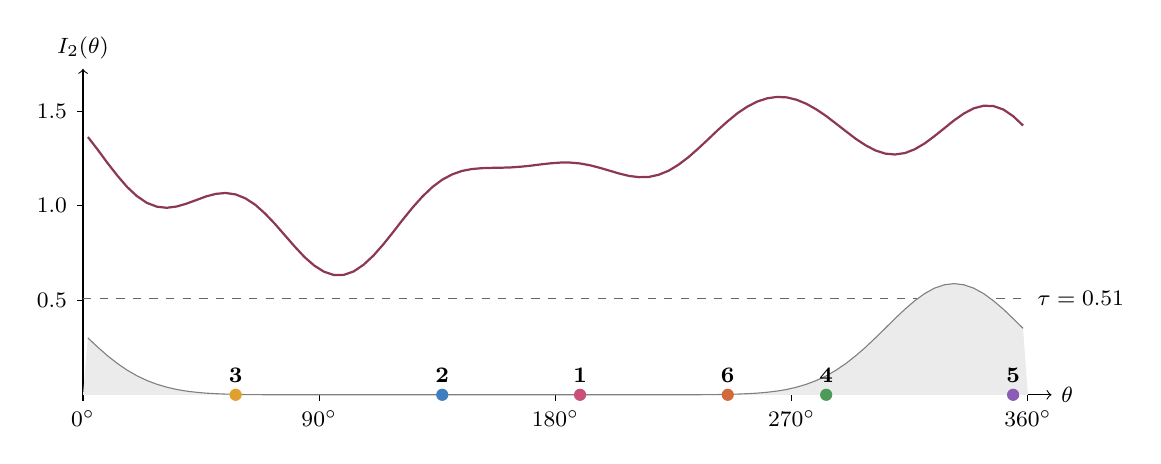
\begin{tikzpicture}[font=\footnotesize]
\definecolor{petA}{HTML}{C8507A}\definecolor{petB}{HTML}{3F7FBF}
\definecolor{petC}{HTML}{E0A030}\definecolor{petD}{HTML}{4E9A5B}
\definecolor{petE}{HTML}{8A5CB8}\definecolor{petF}{HTML}{D2693C}
\definecolor{petG}{HTML}{3AA6A0}\definecolor{petH}{HTML}{8C8C3A}
\draw[->] (0,0) -- (12.30,0) node[right] {$\theta$};
\draw[->] (0,0) -- (0,4.14) node[above] {$I_2(\theta)$};
\draw (0.000,0) -- (0.000,-0.08) node[below] {$0^\circ$};
\draw (3.000,0) -- (3.000,-0.08) node[below] {$90^\circ$};
\draw (6.000,0) -- (6.000,-0.08) node[below] {$180^\circ$};
\draw (9.000,0) -- (9.000,-0.08) node[below] {$270^\circ$};
\draw (12.000,0) -- (12.000,-0.08) node[below] {$360^\circ$};
\draw (0,1.200) -- (-0.08,1.200) node[left] {0.5};
\draw (0,2.400) -- (-0.08,2.400) node[left] {1.0};
\draw (0,3.600) -- (-0.08,3.600) node[left] {1.5};
\draw[black!60, dashed] (0,1.221) -- (12.000,1.221) node[right, black] {$\tau=0.51$};
\fill[black!8] plot coordinates {(0.062,0.722) (0.188,0.604) (0.312,0.495) (0.438,0.397) (0.562,0.312) (0.688,0.240) (0.812,0.181) (0.938,0.134) (1.062,0.097) (1.188,0.068) (1.312,0.047) (1.438,0.032) (1.562,0.021) (1.688,0.014) (1.812,0.009) (1.938,0.006) (2.062,0.003) (2.188,0.002) (2.312,0.001) (2.438,0.001) (2.562,0.000) (2.688,0.000) (2.812,0.000) (2.938,0.000) (3.062,0.000) (3.188,0.000) (3.312,0.000) (3.438,0.000) (3.562,0.000) (3.688,0.000) (3.812,0.000) (3.938,0.000) (4.062,0.000) (4.188,0.000) (4.312,0.000) (4.438,0.000) (4.562,0.000) (4.688,0.000) (4.812,0.000) (4.938,0.000) (5.062,0.000) (5.188,0.000) (5.312,0.000) (5.438,0.000) (5.562,0.000) (5.688,0.000) (5.812,0.000) (5.938,0.000) (6.062,0.000) (6.188,0.000) (6.312,0.000) (6.438,0.000) (6.562,0.000) (6.688,0.000) (6.812,0.000) (6.938,0.000) (7.062,0.000) (7.188,0.000) (7.312,0.000) (7.438,0.000) (7.562,0.000) (7.688,0.001) (7.812,0.001) (7.938,0.002) (8.062,0.003) (8.188,0.006) (8.312,0.009) (8.438,0.014) (8.562,0.021) (8.688,0.032) (8.812,0.047) (8.938,0.068) (9.062,0.097) (9.188,0.134) (9.312,0.181) (9.438,0.240) (9.562,0.312) (9.688,0.397) (9.812,0.495) (9.938,0.604) (10.062,0.722) (10.188,0.845) (10.312,0.968) (10.438,1.087) (10.562,1.194) (10.688,1.285) (10.812,1.354) (10.938,1.397) (11.062,1.412) (11.188,1.397) (11.312,1.354) (11.438,1.285) (11.562,1.194) (11.688,1.087) (11.812,0.968) (11.938,0.845)} -- (12.000,0) -- (0,0) -- cycle;
\draw[black!50] plot coordinates {(0.062,0.722) (0.188,0.604) (0.312,0.495) (0.438,0.397) (0.562,0.312) (0.688,0.240) (0.812,0.181) (0.938,0.134) (1.062,0.097) (1.188,0.068) (1.312,0.047) (1.438,0.032) (1.562,0.021) (1.688,0.014) (1.812,0.009) (1.938,0.006) (2.062,0.003) (2.188,0.002) (2.312,0.001) (2.438,0.001) (2.562,0.000) (2.688,0.000) (2.812,0.000) (2.938,0.000) (3.062,0.000) (3.188,0.000) (3.312,0.000) (3.438,0.000) (3.562,0.000) (3.688,0.000) (3.812,0.000) (3.938,0.000) (4.062,0.000) (4.188,0.000) (4.312,0.000) (4.438,0.000) (4.562,0.000) (4.688,0.000) (4.812,0.000) (4.938,0.000) (5.062,0.000) (5.188,0.000) (5.312,0.000) (5.438,0.000) (5.562,0.000) (5.688,0.000) (5.812,0.000) (5.938,0.000) (6.062,0.000) (6.188,0.000) (6.312,0.000) (6.438,0.000) (6.562,0.000) (6.688,0.000) (6.812,0.000) (6.938,0.000) (7.062,0.000) (7.188,0.000) (7.312,0.000) (7.438,0.000) (7.562,0.000) (7.688,0.001) (7.812,0.001) (7.938,0.002) (8.062,0.003) (8.188,0.006) (8.312,0.009) (8.438,0.014) (8.562,0.021) (8.688,0.032) (8.812,0.047) (8.938,0.068) (9.062,0.097) (9.188,0.134) (9.312,0.181) (9.438,0.240) (9.562,0.312) (9.688,0.397) (9.812,0.495) (9.938,0.604) (10.062,0.722) (10.188,0.845) (10.312,0.968) (10.438,1.087) (10.562,1.194) (10.688,1.285) (10.812,1.354) (10.938,1.397) (11.062,1.412) (11.188,1.397) (11.312,1.354) (11.438,1.285) (11.562,1.194) (11.688,1.087) (11.812,0.968) (11.938,0.845)};
\draw[thick, petA!70!black] plot coordinates {(0.062,3.274) (0.188,3.111) (0.312,2.942) (0.438,2.781) (0.562,2.637) (0.688,2.520) (0.812,2.437) (0.938,2.389) (1.062,2.375) (1.188,2.391) (1.312,2.427) (1.438,2.473) (1.562,2.519) (1.688,2.552) (1.812,2.563) (1.938,2.545) (2.062,2.495) (2.188,2.413) (2.312,2.302) (2.438,2.170) (2.562,2.027) (2.688,1.883) (2.812,1.750) (2.938,1.640) (3.062,1.562) (3.188,1.521) (3.312,1.523) (3.438,1.567) (3.562,1.651) (3.688,1.768) (3.812,1.909) (3.938,2.066) (4.062,2.226) (4.188,2.381) (4.312,2.520) (4.438,2.639) (4.562,2.732) (4.688,2.799) (4.812,2.843) (4.938,2.867) (5.062,2.878) (5.188,2.882) (5.312,2.884) (5.438,2.888) (5.562,2.897) (5.688,2.910) (5.812,2.926) (5.938,2.940) (6.062,2.949) (6.188,2.949) (6.312,2.938) (6.438,2.915) (6.562,2.883) (6.688,2.846) (6.812,2.809) (6.938,2.779) (7.062,2.764) (7.188,2.767) (7.312,2.795) (7.438,2.846) (7.562,2.922) (7.688,3.017) (7.812,3.126) (7.938,3.244) (8.062,3.362) (8.188,3.475) (8.312,3.576) (8.438,3.660) (8.562,3.724) (8.688,3.765) (8.812,3.783) (8.938,3.777) (9.062,3.747) (9.188,3.695) (9.312,3.625) (9.438,3.540) (9.562,3.445) (9.688,3.347) (9.812,3.252) (9.938,3.169) (10.062,3.104) (10.188,3.063) (10.312,3.052) (10.438,3.070) (10.562,3.118) (10.688,3.192) (10.812,3.284) (10.938,3.385) (11.062,3.485) (11.188,3.573) (11.312,3.638) (11.438,3.671) (11.562,3.667) (11.688,3.623) (11.812,3.539) (11.938,3.420)};
\fill[petA] (6.312,0) circle (2.2pt); \node[above, inner sep=1pt] at (6.312,0.12) {\textbf{1}};
\fill[petB] (4.562,0) circle (2.2pt); \node[above, inner sep=1pt] at (4.562,0.12) {\textbf{2}};
\fill[petC] (1.938,0) circle (2.2pt); \node[above, inner sep=1pt] at (1.938,0.12) {\textbf{3}};
\fill[petD] (9.438,0) circle (2.2pt); \node[above, inner sep=1pt] at (9.438,0.12) {\textbf{4}};
\fill[petE] (11.812,0) circle (2.2pt); \node[above, inner sep=1pt] at (11.812,0.12) {\textbf{5}};
\fill[petF] (8.188,0) circle (2.2pt); \node[above, inner sep=1pt] at (8.188,0.12) {\textbf{6}};
\end{tikzpicture}

\caption{Row-0 inhibition on layer 2 of seed 11. Grey: the stagger term from
layer 1's single petal, before layer 2 has any primordia. Red: the total after
initiation. Dots: the six primordia, numbered in the order they appeared. The
dashed line is the threshold $\tau$; a cell can only initiate below it.}
\label{fig:ca-inhibition}
\end{figure}

\paragraph{Growth on layer 2.} \Cref{fig:ca-sweeps} shows the grid unrolled:
azimuth left to right from $0^\circ$ to $360^\circ$, row 0 at the bottom, one
colour per petal, primordia outlined. After 3 sweeps each petal is a short
stub; after 8 sweeps they are mounds of 43 to 56 cells; by sweep 15 the mounds
have met their neighbours near the base and keep rising; by sweep 25 almost
every row up to the caps is closed. Sweep 31 is the last one that changes
anything; sweep 32 changes nothing and, being past the 29th, ends the phase
with 1991 of 2688 cells owned. The petal at $354^\circ$ wraps across the $0^\circ$ seam,
which is why it appears at both edges. The resulting petals:
\begin{center}\small
\begin{tabular}{@{}cccccc@{}}
\toprule
Base angle & Cap $H_j$ & Cells & Rows reached & Span on row 0 & Widest row \\
\midrule
$58^\circ$ & 20 & 385 & 20 & $71^\circ$ & $79^\circ$ \\
$137^\circ$ & 20 & 359 & 20 & $64^\circ$ & $71^\circ$ \\
$189^\circ$ & 21 & 312 & 21 & $60^\circ$ & $64^\circ$ \\
$246^\circ$ & 22 & 258 & 22 & $41^\circ$ & $52^\circ$ \\
$283^\circ$ & 21 & 310 & 21 & $56^\circ$ & $64^\circ$ \\
$354^\circ$ & 21 & 367 & 21 & $68^\circ$ & $79^\circ$ \\
\bottomrule
\end{tabular}
\end{center}
The petal at $246^\circ$ is the narrowest because it started last, in the
smallest gap; the petal at $58^\circ$ is the widest because it had the most
room. Every petal reached its cap, so their heights are exactly the drawn
$H_j$.

\begin{figure}[ht]
\centering
% Generated by tools/ca_figures.py from seed 11, flower 0. Do not edit.
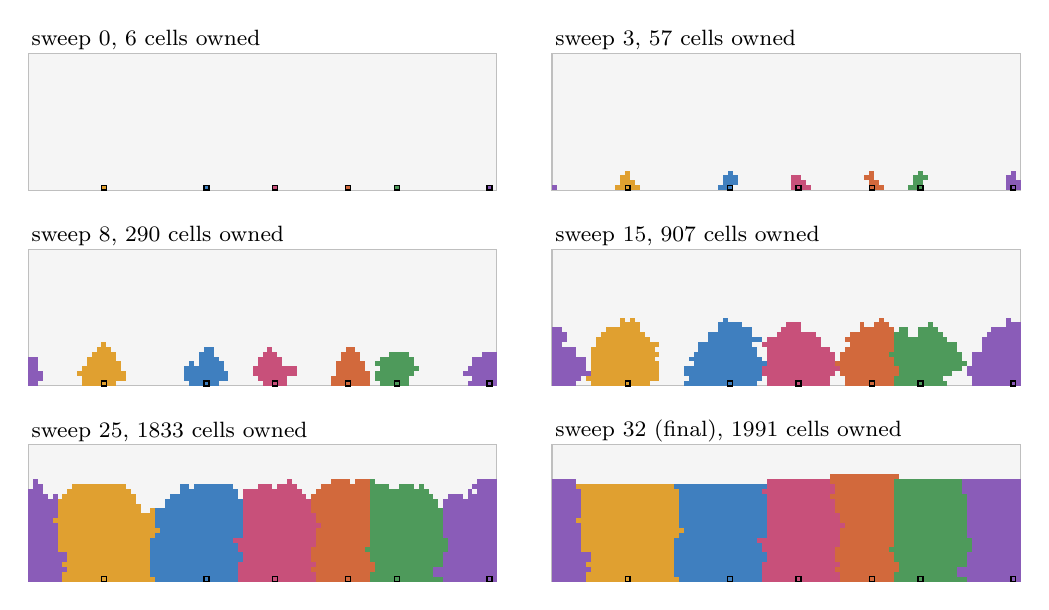
\begin{tikzpicture}[font=\footnotesize]
\definecolor{petA}{HTML}{C8507A}\definecolor{petB}{HTML}{3F7FBF}
\definecolor{petC}{HTML}{E0A030}\definecolor{petD}{HTML}{4E9A5B}
\definecolor{petE}{HTML}{8A5CB8}\definecolor{petF}{HTML}{D2693C}
\definecolor{petG}{HTML}{3AA6A0}\definecolor{petH}{HTML}{8C8C3A}
\draw[black!25, fill=black!4] (0.000,0.000) rectangle (5.952,1.736);
\fill[petC] (0.930,0.000) rectangle (0.992,0.062);
\fill[petB] (2.232,0.000) rectangle (2.294,0.062);
\fill[petA] (3.100,0.000) rectangle (3.162,0.062);
\fill[petF] (4.030,0.000) rectangle (4.092,0.062);
\fill[petD] (4.650,0.000) rectangle (4.712,0.062);
\fill[petE] (5.828,0.000) rectangle (5.890,0.062);
\draw[black, line width=0.5pt] (3.100,0.000) rectangle (3.162,0.062);
\draw[black, line width=0.5pt] (2.232,0.000) rectangle (2.294,0.062);
\draw[black, line width=0.5pt] (0.930,0.000) rectangle (0.992,0.062);
\draw[black, line width=0.5pt] (4.650,0.000) rectangle (4.712,0.062);
\draw[black, line width=0.5pt] (5.828,0.000) rectangle (5.890,0.062);
\draw[black, line width=0.5pt] (4.030,0.000) rectangle (4.092,0.062);
\node[above right, inner sep=1pt] at (0.000,1.736) {sweep 0, 6 cells owned};
\draw[black!25, fill=black!4] (6.652,0.000) rectangle (12.604,1.736);
\fill[petE] (6.652,0.000) rectangle (6.714,0.062);
\fill[petC] (7.458,0.000) rectangle (7.768,0.062);
\fill[petB] (8.760,0.000) rectangle (8.946,0.062);
\fill[petA] (9.690,0.000) rectangle (9.938,0.062);
\fill[petF] (10.682,0.000) rectangle (10.868,0.062);
\fill[petD] (11.178,0.000) rectangle (11.364,0.062);
\fill[petE] (12.418,0.000) rectangle (12.604,0.062);
\fill[petC] (7.520,0.062) rectangle (7.706,0.124);
\fill[petB] (8.822,0.062) rectangle (9.008,0.124);
\fill[petA] (9.690,0.062) rectangle (9.876,0.124);
\fill[petF] (10.682,0.062) rectangle (10.806,0.124);
\fill[petD] (11.240,0.062) rectangle (11.364,0.124);
\fill[petE] (12.418,0.062) rectangle (12.604,0.124);
\fill[petC] (7.520,0.124) rectangle (7.644,0.186);
\fill[petB] (8.822,0.124) rectangle (9.008,0.186);
\fill[petA] (9.690,0.124) rectangle (9.814,0.186);
\fill[petF] (10.620,0.124) rectangle (10.744,0.186);
\fill[petD] (11.240,0.124) rectangle (11.426,0.186);
\fill[petE] (12.418,0.124) rectangle (12.542,0.186);
\fill[petC] (7.582,0.186) rectangle (7.644,0.248);
\fill[petB] (8.884,0.186) rectangle (8.946,0.248);
\fill[petF] (10.682,0.186) rectangle (10.744,0.248);
\fill[petD] (11.302,0.186) rectangle (11.364,0.248);
\fill[petE] (12.480,0.186) rectangle (12.542,0.248);
\draw[black, line width=0.5pt] (9.752,0.000) rectangle (9.814,0.062);
\draw[black, line width=0.5pt] (8.884,0.000) rectangle (8.946,0.062);
\draw[black, line width=0.5pt] (7.582,0.000) rectangle (7.644,0.062);
\draw[black, line width=0.5pt] (11.302,0.000) rectangle (11.364,0.062);
\draw[black, line width=0.5pt] (12.480,0.000) rectangle (12.542,0.062);
\draw[black, line width=0.5pt] (10.682,0.000) rectangle (10.744,0.062);
\node[above right, inner sep=1pt] at (6.652,1.736) {sweep 3, 57 cells owned};
\draw[black!25, fill=black!4] (0.000,-2.486) rectangle (5.952,-0.750);
\fill[petE] (0.000,-2.486) rectangle (0.124,-2.424);
\fill[petC] (0.682,-2.486) rectangle (1.116,-2.424);
\fill[petB] (2.046,-2.486) rectangle (2.418,-2.424);
\fill[petA] (2.976,-2.486) rectangle (3.286,-2.424);
\fill[petF] (3.844,-2.486) rectangle (4.340,-2.424);
\fill[petD] (4.464,-2.486) rectangle (4.836,-2.424);
\fill[petE] (5.580,-2.486) rectangle (5.952,-2.424);
\fill[petE] (0.000,-2.424) rectangle (0.186,-2.362);
\fill[petC] (0.682,-2.424) rectangle (1.240,-2.362);
\fill[petB] (1.984,-2.424) rectangle (2.542,-2.362);
\fill[petA] (2.914,-2.424) rectangle (3.286,-2.362);
\fill[petF] (3.844,-2.424) rectangle (4.340,-2.362);
\fill[petD] (4.402,-2.424) rectangle (4.836,-2.362);
\fill[petE] (5.642,-2.424) rectangle (5.952,-2.362);
\fill[petE] (0.000,-2.362) rectangle (0.186,-2.300);
\fill[petC] (0.620,-2.362) rectangle (1.240,-2.300);
\fill[petB] (1.984,-2.362) rectangle (2.542,-2.300);
\fill[petA] (2.852,-2.362) rectangle (3.410,-2.300);
\fill[petF] (3.906,-2.362) rectangle (4.340,-2.300);
\fill[petD] (4.402,-2.362) rectangle (4.898,-2.300);
\fill[petE] (5.518,-2.362) rectangle (5.952,-2.300);
\fill[petE] (0.000,-2.300) rectangle (0.124,-2.238);
\fill[petC] (0.682,-2.300) rectangle (1.178,-2.238);
\fill[petB] (1.984,-2.300) rectangle (2.480,-2.238);
\fill[petA] (2.852,-2.300) rectangle (3.410,-2.238);
\fill[petF] (3.906,-2.300) rectangle (4.278,-2.238);
\fill[petD] (4.464,-2.300) rectangle (4.960,-2.238);
\fill[petE] (5.580,-2.300) rectangle (5.952,-2.238);
\fill[petE] (0.000,-2.238) rectangle (0.124,-2.176);
\fill[petC] (0.744,-2.238) rectangle (1.178,-2.176);
\fill[petB] (2.046,-2.238) rectangle (2.108,-2.176);
\fill[petB] (2.170,-2.238) rectangle (2.480,-2.176);
\fill[petA] (2.914,-2.238) rectangle (3.224,-2.176);
\fill[petF] (3.906,-2.238) rectangle (4.278,-2.176);
\fill[petD] (4.402,-2.238) rectangle (4.898,-2.176);
\fill[petE] (5.642,-2.238) rectangle (5.952,-2.176);
\fill[petE] (0.000,-2.176) rectangle (0.124,-2.114);
\fill[petC] (0.744,-2.176) rectangle (1.116,-2.114);
\fill[petB] (2.170,-2.176) rectangle (2.418,-2.114);
\fill[petA] (2.914,-2.176) rectangle (3.224,-2.114);
\fill[petF] (3.968,-2.176) rectangle (4.216,-2.114);
\fill[petD] (4.464,-2.176) rectangle (4.898,-2.114);
\fill[petE] (5.642,-2.176) rectangle (5.952,-2.114);
\fill[petC] (0.806,-2.114) rectangle (1.116,-2.052);
\fill[petB] (2.170,-2.114) rectangle (2.356,-2.052);
\fill[petA] (2.976,-2.114) rectangle (3.162,-2.052);
\fill[petF] (3.968,-2.114) rectangle (4.216,-2.052);
\fill[petD] (4.588,-2.114) rectangle (4.836,-2.052);
\fill[petE] (5.766,-2.114) rectangle (5.952,-2.052);
\fill[petC] (0.868,-2.052) rectangle (1.054,-1.990);
\fill[petB] (2.232,-2.052) rectangle (2.356,-1.990);
\fill[petA] (3.038,-2.052) rectangle (3.100,-1.990);
\fill[petF] (4.030,-2.052) rectangle (4.154,-1.990);
\fill[petC] (0.930,-1.990) rectangle (0.992,-1.928);
\draw[black, line width=0.5pt] (3.100,-2.486) rectangle (3.162,-2.424);
\draw[black, line width=0.5pt] (2.232,-2.486) rectangle (2.294,-2.424);
\draw[black, line width=0.5pt] (0.930,-2.486) rectangle (0.992,-2.424);
\draw[black, line width=0.5pt] (4.650,-2.486) rectangle (4.712,-2.424);
\draw[black, line width=0.5pt] (5.828,-2.486) rectangle (5.890,-2.424);
\draw[black, line width=0.5pt] (4.030,-2.486) rectangle (4.092,-2.424);
\node[above right, inner sep=1pt] at (0.000,-0.750) {sweep 8, 290 cells owned};
\draw[black!25, fill=black!4] (6.652,-2.486) rectangle (12.604,-0.750);
\fill[petE] (6.652,-2.486) rectangle (6.962,-2.424);
\fill[petC] (7.148,-2.486) rectangle (7.892,-2.424);
\fill[petB] (8.326,-2.486) rectangle (9.256,-2.424);
\fill[petA] (9.380,-2.486) rectangle (10.186,-2.424);
\fill[petF] (10.372,-2.486) rectangle (10.992,-2.424);
\fill[petD] (10.992,-2.486) rectangle (11.674,-2.424);
\fill[petE] (11.984,-2.486) rectangle (12.604,-2.424);
\fill[petE] (6.652,-2.424) rectangle (7.024,-2.362);
\fill[petC] (7.086,-2.424) rectangle (8.016,-2.362);
\fill[petB] (8.388,-2.424) rectangle (9.318,-2.362);
\fill[petA] (9.380,-2.424) rectangle (10.186,-2.362);
\fill[petF] (10.372,-2.424) rectangle (10.992,-2.362);
\fill[petD] (10.992,-2.424) rectangle (11.612,-2.362);
\fill[petE] (11.984,-2.424) rectangle (12.604,-2.362);
\fill[petE] (6.652,-2.362) rectangle (7.148,-2.300);
\fill[petC] (7.148,-2.362) rectangle (8.016,-2.300);
\fill[petB] (8.326,-2.362) rectangle (9.318,-2.300);
\fill[petA] (9.318,-2.362) rectangle (10.248,-2.300);
\fill[petF] (10.310,-2.362) rectangle (11.054,-2.300);
\fill[petD] (11.054,-2.362) rectangle (11.736,-2.300);
\fill[petE] (11.922,-2.362) rectangle (12.604,-2.300);
\fill[petE] (6.652,-2.300) rectangle (7.086,-2.238);
\fill[petC] (7.148,-2.300) rectangle (8.016,-2.238);
\fill[petB] (8.326,-2.300) rectangle (9.318,-2.238);
\fill[petA] (9.318,-2.300) rectangle (10.310,-2.238);
\fill[petF] (10.310,-2.300) rectangle (11.054,-2.238);
\fill[petD] (11.054,-2.300) rectangle (11.860,-2.238);
\fill[petE] (11.922,-2.300) rectangle (12.604,-2.238);
\fill[petE] (6.652,-2.238) rectangle (7.086,-2.176);
\fill[petC] (7.148,-2.238) rectangle (8.016,-2.176);
\fill[petB] (8.450,-2.238) rectangle (9.380,-2.176);
\fill[petA] (9.380,-2.238) rectangle (10.248,-2.176);
\fill[petF] (10.248,-2.238) rectangle (10.992,-2.176);
\fill[petD] (10.992,-2.238) rectangle (11.922,-2.176);
\fill[petE] (11.984,-2.238) rectangle (12.604,-2.176);
\fill[petE] (6.652,-2.176) rectangle (7.086,-2.114);
\fill[petC] (7.148,-2.176) rectangle (7.954,-2.114);
\fill[petB] (8.388,-2.176) rectangle (9.318,-2.114);
\fill[petA] (9.380,-2.176) rectangle (10.248,-2.114);
\fill[petF] (10.310,-2.176) rectangle (10.992,-2.114);
\fill[petD] (10.992,-2.176) rectangle (11.860,-2.114);
\fill[petE] (11.984,-2.176) rectangle (12.604,-2.114);
\fill[petE] (6.652,-2.114) rectangle (6.962,-2.052);
\fill[petC] (7.148,-2.114) rectangle (8.016,-2.052);
\fill[petB] (8.450,-2.114) rectangle (9.256,-2.052);
\fill[petA] (9.380,-2.114) rectangle (10.248,-2.052);
\fill[petF] (10.310,-2.114) rectangle (10.930,-2.052);
\fill[petD] (10.930,-2.114) rectangle (11.860,-2.052);
\fill[petE] (11.984,-2.114) rectangle (12.604,-2.052);
\fill[petE] (6.652,-2.052) rectangle (6.962,-1.990);
\fill[petC] (7.148,-2.052) rectangle (7.954,-1.990);
\fill[petB] (8.512,-2.052) rectangle (9.256,-1.990);
\fill[petA] (9.380,-2.052) rectangle (10.186,-1.990);
\fill[petF] (10.372,-2.052) rectangle (10.992,-1.990);
\fill[petD] (10.992,-2.052) rectangle (11.798,-1.990);
\fill[petE] (12.108,-2.052) rectangle (12.604,-1.990);
\fill[petE] (6.652,-1.990) rectangle (6.776,-1.928);
\fill[petC] (7.210,-1.990) rectangle (8.016,-1.928);
\fill[petB] (8.512,-1.990) rectangle (9.194,-1.928);
\fill[petA] (9.318,-1.990) rectangle (10.062,-1.928);
\fill[petF] (10.434,-1.990) rectangle (10.992,-1.928);
\fill[petD] (10.992,-1.990) rectangle (11.798,-1.928);
\fill[petE] (12.108,-1.990) rectangle (12.604,-1.928);
\fill[petE] (6.652,-1.928) rectangle (6.838,-1.866);
\fill[petC] (7.210,-1.928) rectangle (7.892,-1.866);
\fill[petB] (8.636,-1.928) rectangle (9.318,-1.866);
\fill[petA] (9.380,-1.928) rectangle (10.062,-1.866);
\fill[petF] (10.372,-1.928) rectangle (10.992,-1.866);
\fill[petD] (10.992,-1.928) rectangle (11.674,-1.866);
\fill[petE] (12.108,-1.928) rectangle (12.604,-1.866);
\fill[petE] (6.652,-1.866) rectangle (6.838,-1.804);
\fill[petC] (7.272,-1.866) rectangle (7.830,-1.804);
\fill[petB] (8.636,-1.866) rectangle (9.194,-1.804);
\fill[petA] (9.504,-1.866) rectangle (10.000,-1.804);
\fill[petF] (10.434,-1.866) rectangle (10.992,-1.804);
\fill[petD] (10.992,-1.866) rectangle (11.178,-1.804);
\fill[petD] (11.302,-1.866) rectangle (11.612,-1.804);
\fill[petE] (12.170,-1.866) rectangle (12.604,-1.804);
\fill[petE] (6.652,-1.804) rectangle (6.776,-1.742);
\fill[petC] (7.334,-1.804) rectangle (7.768,-1.742);
\fill[petB] (8.760,-1.804) rectangle (9.194,-1.742);
\fill[petA] (9.566,-1.804) rectangle (9.814,-1.742);
\fill[petF] (10.558,-1.804) rectangle (10.992,-1.742);
\fill[petD] (11.054,-1.804) rectangle (11.178,-1.742);
\fill[petD] (11.302,-1.804) rectangle (11.550,-1.742);
\fill[petE] (12.232,-1.804) rectangle (12.604,-1.742);
\fill[petC] (7.520,-1.742) rectangle (7.768,-1.680);
\fill[petB] (8.760,-1.742) rectangle (9.070,-1.680);
\fill[petA] (9.628,-1.742) rectangle (9.814,-1.680);
\fill[petF] (10.558,-1.742) rectangle (10.620,-1.680);
\fill[petF] (10.744,-1.742) rectangle (10.930,-1.680);
\fill[petD] (11.426,-1.742) rectangle (11.488,-1.680);
\fill[petE] (12.418,-1.742) rectangle (12.604,-1.680);
\fill[petC] (7.520,-1.680) rectangle (7.582,-1.618);
\fill[petC] (7.644,-1.680) rectangle (7.706,-1.618);
\fill[petB] (8.822,-1.680) rectangle (8.884,-1.618);
\fill[petF] (10.806,-1.680) rectangle (10.868,-1.618);
\fill[petE] (12.418,-1.680) rectangle (12.480,-1.618);
\draw[black, line width=0.5pt] (9.752,-2.486) rectangle (9.814,-2.424);
\draw[black, line width=0.5pt] (8.884,-2.486) rectangle (8.946,-2.424);
\draw[black, line width=0.5pt] (7.582,-2.486) rectangle (7.644,-2.424);
\draw[black, line width=0.5pt] (11.302,-2.486) rectangle (11.364,-2.424);
\draw[black, line width=0.5pt] (12.480,-2.486) rectangle (12.542,-2.424);
\draw[black, line width=0.5pt] (10.682,-2.486) rectangle (10.744,-2.424);
\node[above right, inner sep=1pt] at (6.652,-0.750) {sweep 15, 907 cells owned};
\draw[black!25, fill=black!4] (0.000,-4.972) rectangle (5.952,-3.236);
\fill[petE] (0.000,-4.972) rectangle (0.434,-4.910);
\fill[petC] (0.434,-4.972) rectangle (1.612,-4.910);
\fill[petB] (1.612,-4.972) rectangle (2.666,-4.910);
\fill[petA] (2.666,-4.972) rectangle (3.658,-4.910);
\fill[petF] (3.658,-4.972) rectangle (4.340,-4.910);
\fill[petD] (4.340,-4.972) rectangle (5.270,-4.910);
\fill[petE] (5.270,-4.972) rectangle (5.952,-4.910);
\fill[petE] (0.000,-4.910) rectangle (0.434,-4.848);
\fill[petC] (0.434,-4.910) rectangle (1.550,-4.848);
\fill[petB] (1.550,-4.910) rectangle (2.666,-4.848);
\fill[petA] (2.666,-4.910) rectangle (3.658,-4.848);
\fill[petF] (3.658,-4.910) rectangle (4.340,-4.848);
\fill[petD] (4.340,-4.910) rectangle (5.146,-4.848);
\fill[petE] (5.146,-4.910) rectangle (5.952,-4.848);
\fill[petE] (0.000,-4.848) rectangle (0.496,-4.786);
\fill[petC] (0.496,-4.848) rectangle (1.550,-4.786);
\fill[petB] (1.550,-4.848) rectangle (2.666,-4.786);
\fill[petA] (2.666,-4.848) rectangle (3.596,-4.786);
\fill[petF] (3.596,-4.848) rectangle (4.402,-4.786);
\fill[petD] (4.402,-4.848) rectangle (5.146,-4.786);
\fill[petE] (5.146,-4.848) rectangle (5.952,-4.786);
\fill[petE] (0.000,-4.786) rectangle (0.434,-4.724);
\fill[petC] (0.434,-4.786) rectangle (1.550,-4.724);
\fill[petB] (1.550,-4.786) rectangle (2.666,-4.724);
\fill[petA] (2.666,-4.786) rectangle (3.658,-4.724);
\fill[petF] (3.658,-4.786) rectangle (4.402,-4.724);
\fill[petD] (4.402,-4.786) rectangle (5.270,-4.724);
\fill[petE] (5.270,-4.786) rectangle (5.952,-4.724);
\fill[petE] (0.000,-4.724) rectangle (0.496,-4.662);
\fill[petC] (0.496,-4.724) rectangle (1.550,-4.662);
\fill[petB] (1.550,-4.724) rectangle (2.728,-4.662);
\fill[petA] (2.728,-4.724) rectangle (3.596,-4.662);
\fill[petF] (3.596,-4.724) rectangle (4.340,-4.662);
\fill[petD] (4.340,-4.724) rectangle (5.270,-4.662);
\fill[petE] (5.270,-4.724) rectangle (5.952,-4.662);
\fill[petE] (0.000,-4.662) rectangle (0.496,-4.600);
\fill[petC] (0.496,-4.662) rectangle (1.550,-4.600);
\fill[petB] (1.550,-4.662) rectangle (2.728,-4.600);
\fill[petA] (2.728,-4.662) rectangle (3.596,-4.600);
\fill[petF] (3.596,-4.662) rectangle (4.340,-4.600);
\fill[petD] (4.340,-4.662) rectangle (5.270,-4.600);
\fill[petE] (5.270,-4.662) rectangle (5.952,-4.600);
\fill[petE] (0.000,-4.600) rectangle (0.372,-4.538);
\fill[petC] (0.372,-4.600) rectangle (1.550,-4.538);
\fill[petB] (1.550,-4.600) rectangle (2.666,-4.538);
\fill[petA] (2.666,-4.600) rectangle (3.596,-4.538);
\fill[petF] (3.596,-4.600) rectangle (4.278,-4.538);
\fill[petD] (4.278,-4.600) rectangle (5.332,-4.538);
\fill[petE] (5.332,-4.600) rectangle (5.952,-4.538);
\fill[petE] (0.000,-4.538) rectangle (0.372,-4.476);
\fill[petC] (0.372,-4.538) rectangle (1.550,-4.476);
\fill[petB] (1.550,-4.538) rectangle (2.666,-4.476);
\fill[petA] (2.666,-4.538) rectangle (3.658,-4.476);
\fill[petF] (3.658,-4.538) rectangle (4.340,-4.476);
\fill[petD] (4.340,-4.538) rectangle (5.332,-4.476);
\fill[petE] (5.332,-4.538) rectangle (5.952,-4.476);
\fill[petE] (0.000,-4.476) rectangle (0.372,-4.414);
\fill[petC] (0.372,-4.476) rectangle (1.550,-4.414);
\fill[petB] (1.550,-4.476) rectangle (2.604,-4.414);
\fill[petA] (2.604,-4.476) rectangle (3.658,-4.414);
\fill[petF] (3.658,-4.476) rectangle (4.340,-4.414);
\fill[petD] (4.340,-4.476) rectangle (5.332,-4.414);
\fill[petE] (5.332,-4.476) rectangle (5.952,-4.414);
\fill[petE] (0.000,-4.414) rectangle (0.372,-4.352);
\fill[petC] (0.372,-4.414) rectangle (1.612,-4.352);
\fill[petB] (1.612,-4.414) rectangle (2.728,-4.352);
\fill[petA] (2.728,-4.414) rectangle (3.658,-4.352);
\fill[petF] (3.658,-4.414) rectangle (4.340,-4.352);
\fill[petD] (4.340,-4.414) rectangle (5.270,-4.352);
\fill[petE] (5.270,-4.414) rectangle (5.952,-4.352);
\fill[petE] (0.000,-4.352) rectangle (0.372,-4.290);
\fill[petC] (0.372,-4.352) rectangle (1.674,-4.290);
\fill[petB] (1.674,-4.352) rectangle (2.728,-4.290);
\fill[petA] (2.728,-4.352) rectangle (3.658,-4.290);
\fill[petF] (3.658,-4.352) rectangle (4.340,-4.290);
\fill[petD] (4.340,-4.352) rectangle (5.270,-4.290);
\fill[petE] (5.270,-4.352) rectangle (5.952,-4.290);
\fill[petE] (0.000,-4.290) rectangle (0.372,-4.228);
\fill[petC] (0.372,-4.290) rectangle (1.612,-4.228);
\fill[petB] (1.612,-4.290) rectangle (2.728,-4.228);
\fill[petA] (2.728,-4.290) rectangle (3.720,-4.228);
\fill[petF] (3.720,-4.290) rectangle (4.340,-4.228);
\fill[petD] (4.340,-4.290) rectangle (5.270,-4.228);
\fill[petE] (5.270,-4.290) rectangle (5.952,-4.228);
\fill[petE] (0.000,-4.228) rectangle (0.310,-4.166);
\fill[petC] (0.310,-4.228) rectangle (1.612,-4.166);
\fill[petB] (1.612,-4.228) rectangle (2.728,-4.166);
\fill[petA] (2.728,-4.228) rectangle (3.658,-4.166);
\fill[petF] (3.658,-4.228) rectangle (4.340,-4.166);
\fill[petD] (4.340,-4.228) rectangle (5.270,-4.166);
\fill[petE] (5.270,-4.228) rectangle (5.952,-4.166);
\fill[petE] (0.000,-4.166) rectangle (0.372,-4.104);
\fill[petC] (0.372,-4.166) rectangle (1.612,-4.104);
\fill[petB] (1.612,-4.166) rectangle (2.728,-4.104);
\fill[petA] (2.728,-4.166) rectangle (3.658,-4.104);
\fill[petF] (3.658,-4.166) rectangle (4.340,-4.104);
\fill[petD] (4.340,-4.166) rectangle (5.270,-4.104);
\fill[petE] (5.270,-4.166) rectangle (5.952,-4.104);
\fill[petE] (0.000,-4.104) rectangle (0.372,-4.042);
\fill[petC] (0.372,-4.104) rectangle (1.426,-4.042);
\fill[petC] (1.550,-4.104) rectangle (1.612,-4.042);
\fill[petB] (1.612,-4.104) rectangle (2.728,-4.042);
\fill[petA] (2.728,-4.104) rectangle (3.596,-4.042);
\fill[petF] (3.596,-4.104) rectangle (4.340,-4.042);
\fill[petD] (4.340,-4.104) rectangle (5.270,-4.042);
\fill[petE] (5.270,-4.104) rectangle (5.952,-4.042);
\fill[petE] (0.000,-4.042) rectangle (0.372,-3.980);
\fill[petC] (0.372,-4.042) rectangle (1.426,-3.980);
\fill[petB] (1.736,-4.042) rectangle (2.728,-3.980);
\fill[petA] (2.728,-4.042) rectangle (3.596,-3.980);
\fill[petF] (3.596,-4.042) rectangle (4.340,-3.980);
\fill[petD] (4.340,-4.042) rectangle (5.208,-3.980);
\fill[petE] (5.270,-4.042) rectangle (5.952,-3.980);
\fill[petE] (0.000,-3.980) rectangle (0.372,-3.918);
\fill[petC] (0.372,-3.980) rectangle (1.364,-3.918);
\fill[petB] (1.736,-3.980) rectangle (2.728,-3.918);
\fill[petA] (2.728,-3.980) rectangle (3.596,-3.918);
\fill[petF] (3.596,-3.980) rectangle (4.340,-3.918);
\fill[petD] (4.340,-3.980) rectangle (5.208,-3.918);
\fill[petE] (5.270,-3.980) rectangle (5.952,-3.918);
\fill[petE] (0.000,-3.918) rectangle (0.248,-3.856);
\fill[petE] (0.310,-3.918) rectangle (0.372,-3.856);
\fill[petC] (0.434,-3.918) rectangle (1.364,-3.856);
\fill[petB] (1.798,-3.918) rectangle (2.666,-3.856);
\fill[petA] (2.728,-3.918) rectangle (3.534,-3.856);
\fill[petF] (3.596,-3.918) rectangle (4.340,-3.856);
\fill[petD] (4.340,-3.918) rectangle (5.146,-3.856);
\fill[petE] (5.332,-3.918) rectangle (5.518,-3.856);
\fill[petE] (5.580,-3.918) rectangle (5.952,-3.856);
\fill[petE] (0.000,-3.856) rectangle (0.186,-3.794);
\fill[petC] (0.496,-3.856) rectangle (1.302,-3.794);
\fill[petB] (1.922,-3.856) rectangle (2.666,-3.794);
\fill[petA] (2.728,-3.856) rectangle (3.472,-3.794);
\fill[petF] (3.658,-3.856) rectangle (4.340,-3.794);
\fill[petD] (4.340,-3.856) rectangle (5.084,-3.794);
\fill[petE] (5.580,-3.856) rectangle (5.642,-3.794);
\fill[petE] (5.704,-3.856) rectangle (5.952,-3.794);
\fill[petE] (0.062,-3.794) rectangle (0.186,-3.732);
\fill[petC] (0.558,-3.794) rectangle (1.240,-3.732);
\fill[petB] (1.922,-3.794) rectangle (2.046,-3.732);
\fill[petB] (2.108,-3.794) rectangle (2.604,-3.732);
\fill[petA] (2.914,-3.794) rectangle (3.100,-3.732);
\fill[petA] (3.162,-3.794) rectangle (3.410,-3.732);
\fill[petF] (3.720,-3.794) rectangle (4.340,-3.732);
\fill[petD] (4.340,-3.794) rectangle (4.588,-3.732);
\fill[petD] (4.712,-3.794) rectangle (4.898,-3.732);
\fill[petD] (4.960,-3.794) rectangle (5.022,-3.732);
\fill[petE] (5.642,-3.794) rectangle (5.952,-3.732);
\fill[petE] (0.062,-3.732) rectangle (0.124,-3.670);
\fill[petA] (3.286,-3.732) rectangle (3.348,-3.670);
\fill[petF] (3.844,-3.732) rectangle (4.092,-3.670);
\fill[petF] (4.154,-3.732) rectangle (4.340,-3.670);
\fill[petD] (4.340,-3.732) rectangle (4.402,-3.670);
\fill[petE] (5.704,-3.732) rectangle (5.952,-3.670);
\draw[black, line width=0.5pt] (3.100,-4.972) rectangle (3.162,-4.910);
\draw[black, line width=0.5pt] (2.232,-4.972) rectangle (2.294,-4.910);
\draw[black, line width=0.5pt] (0.930,-4.972) rectangle (0.992,-4.910);
\draw[black, line width=0.5pt] (4.650,-4.972) rectangle (4.712,-4.910);
\draw[black, line width=0.5pt] (5.828,-4.972) rectangle (5.890,-4.910);
\draw[black, line width=0.5pt] (4.030,-4.972) rectangle (4.092,-4.910);
\node[above right, inner sep=1pt] at (0.000,-3.236) {sweep 25, 1833 cells owned};
\draw[black!25, fill=black!4] (6.652,-4.972) rectangle (12.604,-3.236);
\fill[petE] (6.652,-4.972) rectangle (7.086,-4.910);
\fill[petC] (7.086,-4.972) rectangle (8.264,-4.910);
\fill[petB] (8.264,-4.972) rectangle (9.318,-4.910);
\fill[petA] (9.318,-4.972) rectangle (10.310,-4.910);
\fill[petF] (10.310,-4.972) rectangle (10.992,-4.910);
\fill[petD] (10.992,-4.972) rectangle (11.922,-4.910);
\fill[petE] (11.922,-4.972) rectangle (12.604,-4.910);
\fill[petE] (6.652,-4.910) rectangle (7.086,-4.848);
\fill[petC] (7.086,-4.910) rectangle (8.202,-4.848);
\fill[petB] (8.202,-4.910) rectangle (9.318,-4.848);
\fill[petA] (9.318,-4.910) rectangle (10.310,-4.848);
\fill[petF] (10.310,-4.910) rectangle (10.992,-4.848);
\fill[petD] (10.992,-4.910) rectangle (11.798,-4.848);
\fill[petE] (11.798,-4.910) rectangle (12.604,-4.848);
\fill[petE] (6.652,-4.848) rectangle (7.148,-4.786);
\fill[petC] (7.148,-4.848) rectangle (8.202,-4.786);
\fill[petB] (8.202,-4.848) rectangle (9.318,-4.786);
\fill[petA] (9.318,-4.848) rectangle (10.248,-4.786);
\fill[petF] (10.248,-4.848) rectangle (11.054,-4.786);
\fill[petD] (11.054,-4.848) rectangle (11.798,-4.786);
\fill[petE] (11.798,-4.848) rectangle (12.604,-4.786);
\fill[petE] (6.652,-4.786) rectangle (7.086,-4.724);
\fill[petC] (7.086,-4.786) rectangle (8.202,-4.724);
\fill[petB] (8.202,-4.786) rectangle (9.318,-4.724);
\fill[petA] (9.318,-4.786) rectangle (10.310,-4.724);
\fill[petF] (10.310,-4.786) rectangle (11.054,-4.724);
\fill[petD] (11.054,-4.786) rectangle (11.922,-4.724);
\fill[petE] (11.922,-4.786) rectangle (12.604,-4.724);
\fill[petE] (6.652,-4.724) rectangle (7.148,-4.662);
\fill[petC] (7.148,-4.724) rectangle (8.202,-4.662);
\fill[petB] (8.202,-4.724) rectangle (9.380,-4.662);
\fill[petA] (9.380,-4.724) rectangle (10.248,-4.662);
\fill[petF] (10.248,-4.724) rectangle (10.992,-4.662);
\fill[petD] (10.992,-4.724) rectangle (11.922,-4.662);
\fill[petE] (11.922,-4.724) rectangle (12.604,-4.662);
\fill[petE] (6.652,-4.662) rectangle (7.148,-4.600);
\fill[petC] (7.148,-4.662) rectangle (8.202,-4.600);
\fill[petB] (8.202,-4.662) rectangle (9.380,-4.600);
\fill[petA] (9.380,-4.662) rectangle (10.248,-4.600);
\fill[petF] (10.248,-4.662) rectangle (10.992,-4.600);
\fill[petD] (10.992,-4.662) rectangle (11.922,-4.600);
\fill[petE] (11.922,-4.662) rectangle (12.604,-4.600);
\fill[petE] (6.652,-4.600) rectangle (7.024,-4.538);
\fill[petC] (7.024,-4.600) rectangle (8.202,-4.538);
\fill[petB] (8.202,-4.600) rectangle (9.318,-4.538);
\fill[petA] (9.318,-4.600) rectangle (10.248,-4.538);
\fill[petF] (10.248,-4.600) rectangle (10.930,-4.538);
\fill[petD] (10.930,-4.600) rectangle (11.984,-4.538);
\fill[petE] (11.984,-4.600) rectangle (12.604,-4.538);
\fill[petE] (6.652,-4.538) rectangle (7.024,-4.476);
\fill[petC] (7.024,-4.538) rectangle (8.202,-4.476);
\fill[petB] (8.202,-4.538) rectangle (9.318,-4.476);
\fill[petA] (9.318,-4.538) rectangle (10.310,-4.476);
\fill[petF] (10.310,-4.538) rectangle (10.992,-4.476);
\fill[petD] (10.992,-4.538) rectangle (11.984,-4.476);
\fill[petE] (11.984,-4.538) rectangle (12.604,-4.476);
\fill[petE] (6.652,-4.476) rectangle (7.024,-4.414);
\fill[petC] (7.024,-4.476) rectangle (8.202,-4.414);
\fill[petB] (8.202,-4.476) rectangle (9.256,-4.414);
\fill[petA] (9.256,-4.476) rectangle (10.310,-4.414);
\fill[petF] (10.310,-4.476) rectangle (10.992,-4.414);
\fill[petD] (10.992,-4.476) rectangle (11.984,-4.414);
\fill[petE] (11.984,-4.476) rectangle (12.604,-4.414);
\fill[petE] (6.652,-4.414) rectangle (7.024,-4.352);
\fill[petC] (7.024,-4.414) rectangle (8.264,-4.352);
\fill[petB] (8.264,-4.414) rectangle (9.380,-4.352);
\fill[petA] (9.380,-4.414) rectangle (10.310,-4.352);
\fill[petF] (10.310,-4.414) rectangle (10.992,-4.352);
\fill[petD] (10.992,-4.414) rectangle (11.922,-4.352);
\fill[petE] (11.922,-4.414) rectangle (12.604,-4.352);
\fill[petE] (6.652,-4.352) rectangle (7.024,-4.290);
\fill[petC] (7.024,-4.352) rectangle (8.326,-4.290);
\fill[petB] (8.326,-4.352) rectangle (9.380,-4.290);
\fill[petA] (9.380,-4.352) rectangle (10.310,-4.290);
\fill[petF] (10.310,-4.352) rectangle (10.992,-4.290);
\fill[petD] (10.992,-4.352) rectangle (11.922,-4.290);
\fill[petE] (11.922,-4.352) rectangle (12.604,-4.290);
\fill[petE] (6.652,-4.290) rectangle (7.024,-4.228);
\fill[petC] (7.024,-4.290) rectangle (8.264,-4.228);
\fill[petB] (8.264,-4.290) rectangle (9.380,-4.228);
\fill[petA] (9.380,-4.290) rectangle (10.372,-4.228);
\fill[petF] (10.372,-4.290) rectangle (10.992,-4.228);
\fill[petD] (10.992,-4.290) rectangle (11.922,-4.228);
\fill[petE] (11.922,-4.290) rectangle (12.604,-4.228);
\fill[petE] (6.652,-4.228) rectangle (6.962,-4.166);
\fill[petC] (6.962,-4.228) rectangle (8.264,-4.166);
\fill[petB] (8.264,-4.228) rectangle (9.380,-4.166);
\fill[petA] (9.380,-4.228) rectangle (10.310,-4.166);
\fill[petF] (10.310,-4.228) rectangle (10.992,-4.166);
\fill[petD] (10.992,-4.228) rectangle (11.922,-4.166);
\fill[petE] (11.922,-4.228) rectangle (12.604,-4.166);
\fill[petE] (6.652,-4.166) rectangle (7.024,-4.104);
\fill[petC] (7.024,-4.166) rectangle (8.264,-4.104);
\fill[petB] (8.264,-4.166) rectangle (9.380,-4.104);
\fill[petA] (9.380,-4.166) rectangle (10.310,-4.104);
\fill[petF] (10.310,-4.166) rectangle (10.992,-4.104);
\fill[petD] (10.992,-4.166) rectangle (11.922,-4.104);
\fill[petE] (11.922,-4.166) rectangle (12.604,-4.104);
\fill[petE] (6.652,-4.104) rectangle (7.024,-4.042);
\fill[petC] (7.024,-4.104) rectangle (8.264,-4.042);
\fill[petB] (8.264,-4.104) rectangle (9.380,-4.042);
\fill[petA] (9.380,-4.104) rectangle (10.248,-4.042);
\fill[petF] (10.248,-4.104) rectangle (10.992,-4.042);
\fill[petD] (10.992,-4.104) rectangle (11.922,-4.042);
\fill[petE] (11.922,-4.104) rectangle (12.604,-4.042);
\fill[petE] (6.652,-4.042) rectangle (7.024,-3.980);
\fill[petC] (7.024,-4.042) rectangle (8.264,-3.980);
\fill[petB] (8.264,-4.042) rectangle (9.380,-3.980);
\fill[petA] (9.380,-4.042) rectangle (10.248,-3.980);
\fill[petF] (10.248,-4.042) rectangle (10.992,-3.980);
\fill[petD] (10.992,-4.042) rectangle (11.922,-3.980);
\fill[petE] (11.922,-4.042) rectangle (12.604,-3.980);
\fill[petE] (6.652,-3.980) rectangle (7.024,-3.918);
\fill[petC] (7.024,-3.980) rectangle (8.264,-3.918);
\fill[petB] (8.264,-3.980) rectangle (9.380,-3.918);
\fill[petA] (9.380,-3.980) rectangle (10.248,-3.918);
\fill[petF] (10.248,-3.980) rectangle (10.992,-3.918);
\fill[petD] (10.992,-3.980) rectangle (11.922,-3.918);
\fill[petE] (11.922,-3.980) rectangle (12.604,-3.918);
\fill[petE] (6.652,-3.918) rectangle (7.024,-3.856);
\fill[petC] (7.024,-3.918) rectangle (8.264,-3.856);
\fill[petB] (8.264,-3.918) rectangle (9.380,-3.856);
\fill[petA] (9.380,-3.918) rectangle (10.186,-3.856);
\fill[petF] (10.186,-3.918) rectangle (10.992,-3.856);
\fill[petD] (10.992,-3.918) rectangle (11.922,-3.856);
\fill[petE] (11.922,-3.918) rectangle (12.604,-3.856);
\fill[petE] (6.652,-3.856) rectangle (7.024,-3.794);
\fill[petC] (7.024,-3.856) rectangle (8.264,-3.794);
\fill[petB] (8.264,-3.856) rectangle (9.318,-3.794);
\fill[petA] (9.318,-3.856) rectangle (10.248,-3.794);
\fill[petF] (10.248,-3.856) rectangle (10.992,-3.794);
\fill[petD] (10.992,-3.856) rectangle (11.860,-3.794);
\fill[petE] (11.860,-3.856) rectangle (12.604,-3.794);
\fill[petE] (6.652,-3.794) rectangle (6.962,-3.732);
\fill[petC] (6.962,-3.794) rectangle (8.202,-3.732);
\fill[petB] (8.202,-3.794) rectangle (9.380,-3.732);
\fill[petA] (9.380,-3.794) rectangle (10.248,-3.732);
\fill[petF] (10.248,-3.794) rectangle (10.992,-3.732);
\fill[petD] (10.992,-3.794) rectangle (11.860,-3.732);
\fill[petE] (11.860,-3.794) rectangle (12.604,-3.732);
\fill[petE] (6.652,-3.732) rectangle (6.962,-3.670);
\fill[petA] (9.380,-3.732) rectangle (10.186,-3.670);
\fill[petF] (10.186,-3.732) rectangle (10.992,-3.670);
\fill[petD] (10.992,-3.732) rectangle (11.860,-3.670);
\fill[petE] (11.860,-3.732) rectangle (12.604,-3.670);
\fill[petF] (10.186,-3.670) rectangle (11.054,-3.608);
\draw[black, line width=0.5pt] (9.752,-4.972) rectangle (9.814,-4.910);
\draw[black, line width=0.5pt] (8.884,-4.972) rectangle (8.946,-4.910);
\draw[black, line width=0.5pt] (7.582,-4.972) rectangle (7.644,-4.910);
\draw[black, line width=0.5pt] (11.302,-4.972) rectangle (11.364,-4.910);
\draw[black, line width=0.5pt] (12.480,-4.972) rectangle (12.542,-4.910);
\draw[black, line width=0.5pt] (10.682,-4.972) rectangle (10.744,-4.910);
\node[above right, inner sep=1pt] at (6.652,-3.236) {sweep 32 (final), 1991 cells owned};
\end{tikzpicture}

\caption{The growth phase on layer 2 of seed 11, at six moments. Each panel is
the $96\times28$ grid unrolled (azimuth across, row 0 at the bottom); colours
are petals, outlined cells are the primordia, grey is empty.}
\label{fig:ca-sweeps}
\end{figure}

\paragraph{All ten layers.} Running the same two phases on every shell gives
\begin{center}\small
\begin{tabular}{@{}cccccc@{}}
\toprule
Layer & $a_k$ & Row-0 cells free of stagger & Petals & Sweeps & Cells owned \\
\midrule
0 & 0.927 & 96 & 6 & 34 & 73\% \\
1 & 1.020 & 8 & 1 & 84 & 73\% \\
2 & 1.113 & 89 & 6 & 32 & 74\% \\
3 & 1.207 & 26 & 3 & 80 & 82\% \\
4 & 1.300 & 75 & 5 & 43 & 84\% \\
5 & 1.393 & 58 & 6 & 68 & 88\% \\
6 & 1.486 & 49 & 5 & 55 & 89\% \\
7 & 1.580 & 69 & 7 & 46 & 88\% \\
8 & 1.673 & 38 & 4 & 58 & 90\% \\
9 & 1.766 & 76 & 8 & 55 & 98\% \\
\bottomrule
\end{tabular}
\end{center}
for 51 petals in all. ``Row-0 cells free of stagger'' counts the cells where
the layer below alone leaves the inhibition under $\tau$, before the layer's
own primordia appear. Three effects from the rules above are visible.
\begin{itemize}[leftmargin=*]
\item \emph{Alternation.} Layer 0's six petals are close to the densest
  spacing for that shell, so their stagger term stays above $\tau$ over all
  but 8 cells of layer 1. Layer 1 gets a single petal. That leaves layer 2
  almost unconstrained (89 free cells), and it gets six again. The counts
  6, 1, 6, 3, 5, 6, 5, 7, 4, 8 follow the free-cell column closely.
\item \emph{More petals outward.} Under the alternation the counts rise, from
  about 4 on the inner layers to about 6 on the outer ones, because the outer
  rings are longer for the same inhibition reach. The owned fraction rises
  too, from 73\% to 98\%, because the caps $H_j$ rise from about 20 rows to
  about 27.
\item \emph{Interleaving.} In \cref{fig:ca-rings}, each layer's primordia tend
  to sit between those of the layer inside it.
\end{itemize}
Layer 1 is the lone-petal case: its one petal spreads around the whole shell
(\cref{fig:ca-layers}), with a row-0 span of $285^\circ$ and $360^\circ$
higher up. Layers with few petals also take longest to settle, because one or two
fronts have to cover the whole ring: layer 3 needs 80 sweeps, and layer 1 is
still growing when the limit of 84 stops it.

\begin{figure}[ht]
\centering
% Generated by tools/ca_figures.py from seed 11, flower 0. Do not edit.
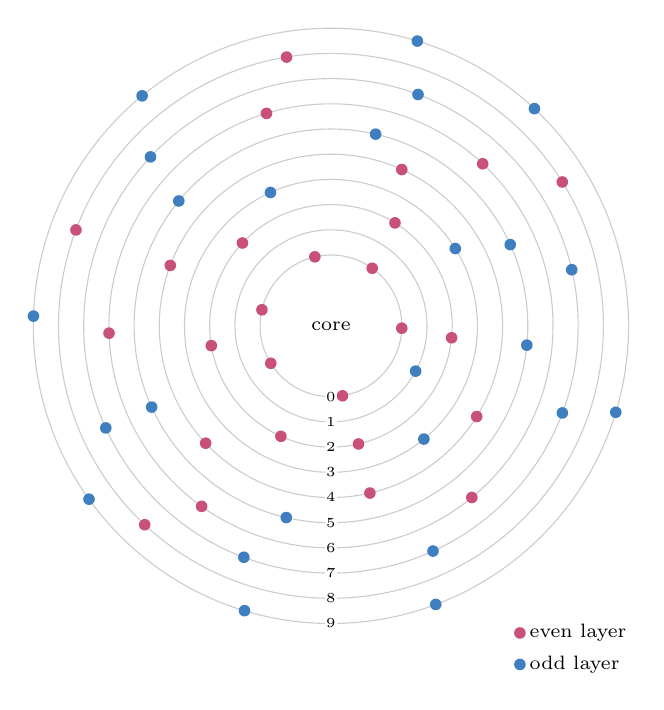
\begin{tikzpicture}[font=\scriptsize]
\definecolor{petA}{HTML}{C8507A}\definecolor{petB}{HTML}{3F7FBF}
\definecolor{petC}{HTML}{E0A030}\definecolor{petD}{HTML}{4E9A5B}
\definecolor{petE}{HTML}{8A5CB8}\definecolor{petF}{HTML}{D2693C}
\definecolor{petG}{HTML}{3AA6A0}\definecolor{petH}{HTML}{8C8C3A}
\draw[black!20] (0,0) circle (0.90);
\fill[petA] (103.12:0.90) circle (2.1pt);
\fill[petA] (279.38:0.90) circle (2.1pt);
\fill[petA] (358.12:0.90) circle (2.1pt);
\fill[petA] (211.88:0.90) circle (2.1pt);
\fill[petA] (166.88:0.90) circle (2.1pt);
\fill[petA] (54.38:0.90) circle (2.1pt);
\node[fill=white, inner sep=0.6pt] at (-90:0.90) {\tiny 0};
\draw[black!20] (0,0) circle (1.22);
\fill[petB] (331.88:1.22) circle (2.1pt);
\node[fill=white, inner sep=0.6pt] at (-90:1.22) {\tiny 1};
\draw[black!20] (0,0) circle (1.54);
\fill[petA] (189.38:1.54) circle (2.1pt);
\fill[petA] (136.88:1.54) circle (2.1pt);
\fill[petA] (58.12:1.54) circle (2.1pt);
\fill[petA] (283.12:1.54) circle (2.1pt);
\fill[petA] (354.38:1.54) circle (2.1pt);
\fill[petA] (245.62:1.54) circle (2.1pt);
\node[fill=white, inner sep=0.6pt] at (-90:1.54) {\tiny 2};
\draw[black!20] (0,0) circle (1.86);
\fill[petB] (309.38:1.86) circle (2.1pt);
\fill[petB] (31.88:1.86) circle (2.1pt);
\fill[petB] (114.38:1.86) circle (2.1pt);
\node[fill=white, inner sep=0.6pt] at (-90:1.86) {\tiny 3};
\draw[black!20] (0,0) circle (2.18);
\fill[petA] (328.12:2.18) circle (2.1pt);
\fill[petA] (159.38:2.18) circle (2.1pt);
\fill[petA] (223.12:2.18) circle (2.1pt);
\fill[petA] (283.12:2.18) circle (2.1pt);
\fill[petA] (65.62:2.18) circle (2.1pt);
\node[fill=white, inner sep=0.6pt] at (-90:2.18) {\tiny 4};
\draw[black!20] (0,0) circle (2.50);
\fill[petB] (354.38:2.50) circle (2.1pt);
\fill[petB] (76.88:2.50) circle (2.1pt);
\fill[petB] (256.88:2.50) circle (2.1pt);
\fill[petB] (140.62:2.50) circle (2.1pt);
\fill[petB] (204.38:2.50) circle (2.1pt);
\fill[petB] (24.38:2.50) circle (2.1pt);
\node[fill=white, inner sep=0.6pt] at (-90:2.50) {\tiny 5};
\draw[black!20] (0,0) circle (2.82);
\fill[petA] (181.88:2.82) circle (2.1pt);
\fill[petA] (309.38:2.82) circle (2.1pt);
\fill[petA] (106.88:2.82) circle (2.1pt);
\fill[petA] (46.88:2.82) circle (2.1pt);
\fill[petA] (234.38:2.82) circle (2.1pt);
\node[fill=white, inner sep=0.6pt] at (-90:2.82) {\tiny 6};
\draw[black!20] (0,0) circle (3.14);
\fill[petB] (294.38:3.14) circle (2.1pt);
\fill[petB] (13.12:3.14) circle (2.1pt);
\fill[petB] (136.88:3.14) circle (2.1pt);
\fill[petB] (69.38:3.14) circle (2.1pt);
\fill[petB] (249.38:3.14) circle (2.1pt);
\fill[petB] (339.38:3.14) circle (2.1pt);
\fill[petB] (204.38:3.14) circle (2.1pt);
\node[fill=white, inner sep=0.6pt] at (-90:3.14) {\tiny 7};
\draw[black!20] (0,0) circle (3.46);
\fill[petA] (99.38:3.46) circle (2.1pt);
\fill[petA] (31.88:3.46) circle (2.1pt);
\fill[petA] (159.38:3.46) circle (2.1pt);
\fill[petA] (226.88:3.46) circle (2.1pt);
\node[fill=white, inner sep=0.6pt] at (-90:3.46) {\tiny 8};
\draw[black!20] (0,0) circle (3.78);
\fill[petB] (129.38:3.78) circle (2.1pt);
\fill[petB] (343.12:3.78) circle (2.1pt);
\fill[petB] (215.62:3.78) circle (2.1pt);
\fill[petB] (178.12:3.78) circle (2.1pt);
\fill[petB] (290.62:3.78) circle (2.1pt);
\fill[petB] (46.88:3.78) circle (2.1pt);
\fill[petB] (73.12:3.78) circle (2.1pt);
\fill[petB] (253.12:3.78) circle (2.1pt);
\node[fill=white, inner sep=0.6pt] at (-90:3.78) {\tiny 9};
\node[align=center] at (0,0) {core};
\fill[petA] (2.4,-3.9) circle (2.1pt) node[right, black] {even layer};
\fill[petB] (2.4,-4.3) circle (2.1pt) node[right, black] {odd layer};
\end{tikzpicture}

\caption{Where the primordia of seed 11 start, one ring per layer seen from
above (layer 0 innermost; ring spacing is schematic). Each layer's
primordia tend to fall in the gaps of the layer inside it.}
\label{fig:ca-rings}
\end{figure}

\begin{figure}[ht]
\centering
% Generated by tools/ca_figures.py from seed 11, flower 0. Do not edit.
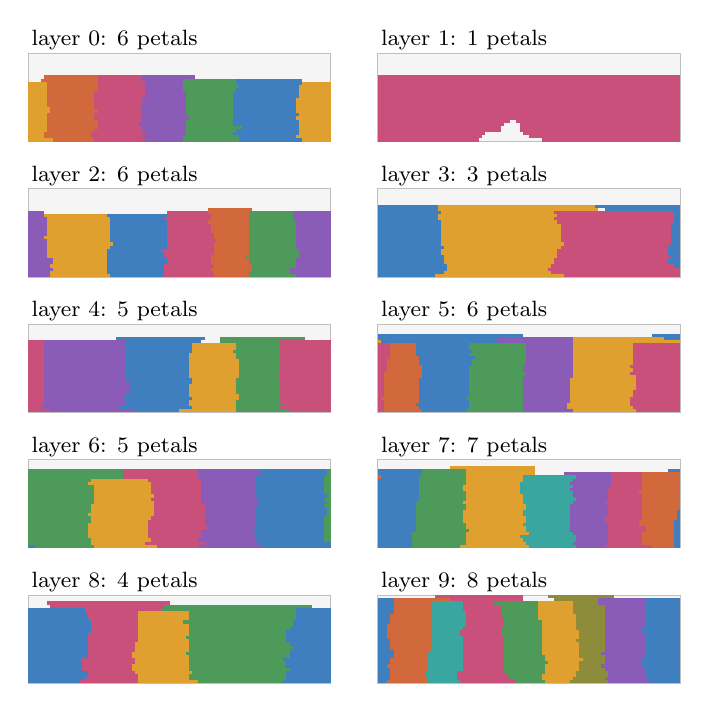
\begin{tikzpicture}[font=\footnotesize]
\definecolor{petA}{HTML}{C8507A}\definecolor{petB}{HTML}{3F7FBF}
\definecolor{petC}{HTML}{E0A030}\definecolor{petD}{HTML}{4E9A5B}
\definecolor{petE}{HTML}{8A5CB8}\definecolor{petF}{HTML}{D2693C}
\definecolor{petG}{HTML}{3AA6A0}\definecolor{petH}{HTML}{8C8C3A}
\draw[black!25, fill=black!4] (0.000,0.000) rectangle (3.840,1.120);
\fill[petC] (0.000,0.000) rectangle (0.320,0.040);
\fill[petF] (0.320,0.000) rectangle (0.840,0.040);
\fill[petA] (0.840,0.000) rectangle (1.480,0.040);
\fill[petE] (1.480,0.000) rectangle (1.960,0.040);
\fill[petD] (1.960,0.000) rectangle (2.680,0.040);
\fill[petB] (2.680,0.000) rectangle (3.480,0.040);
\fill[petC] (3.480,0.000) rectangle (3.840,0.040);
\fill[petC] (0.000,0.040) rectangle (0.200,0.080);
\fill[petF] (0.200,0.040) rectangle (0.800,0.080);
\fill[petA] (0.800,0.040) rectangle (1.440,0.080);
\fill[petE] (1.440,0.040) rectangle (1.960,0.080);
\fill[petD] (1.960,0.040) rectangle (2.680,0.080);
\fill[petB] (2.680,0.040) rectangle (3.400,0.080);
\fill[petC] (3.400,0.040) rectangle (3.840,0.080);
\fill[petC] (0.000,0.080) rectangle (0.200,0.120);
\fill[petF] (0.200,0.080) rectangle (0.800,0.120);
\fill[petA] (0.800,0.080) rectangle (1.480,0.120);
\fill[petE] (1.480,0.080) rectangle (2.000,0.120);
\fill[petD] (2.000,0.080) rectangle (2.600,0.120);
\fill[petB] (2.600,0.080) rectangle (3.440,0.120);
\fill[petC] (3.440,0.080) rectangle (3.840,0.120);
\fill[petC] (0.000,0.120) rectangle (0.240,0.160);
\fill[petF] (0.240,0.120) rectangle (0.840,0.160);
\fill[petA] (0.840,0.120) rectangle (1.440,0.160);
\fill[petE] (1.440,0.120) rectangle (2.000,0.160);
\fill[petD] (2.000,0.120) rectangle (2.640,0.160);
\fill[petB] (2.640,0.120) rectangle (3.440,0.160);
\fill[petC] (3.440,0.120) rectangle (3.840,0.160);
\fill[petC] (0.000,0.160) rectangle (0.240,0.200);
\fill[petF] (0.240,0.160) rectangle (0.880,0.200);
\fill[petA] (0.880,0.160) rectangle (1.440,0.200);
\fill[petE] (1.440,0.160) rectangle (2.000,0.200);
\fill[petD] (2.000,0.160) rectangle (2.720,0.200);
\fill[petB] (2.720,0.160) rectangle (3.440,0.200);
\fill[petC] (3.440,0.160) rectangle (3.840,0.200);
\fill[petC] (0.000,0.200) rectangle (0.240,0.240);
\fill[petF] (0.240,0.200) rectangle (0.880,0.240);
\fill[petA] (0.880,0.200) rectangle (1.400,0.240);
\fill[petE] (1.400,0.200) rectangle (2.000,0.240);
\fill[petD] (2.000,0.200) rectangle (2.600,0.240);
\fill[petB] (2.600,0.200) rectangle (3.440,0.240);
\fill[petC] (3.440,0.200) rectangle (3.840,0.240);
\fill[petC] (0.000,0.240) rectangle (0.240,0.280);
\fill[petF] (0.240,0.240) rectangle (0.880,0.280);
\fill[petA] (0.880,0.240) rectangle (1.440,0.280);
\fill[petE] (1.440,0.240) rectangle (2.000,0.280);
\fill[petD] (2.000,0.240) rectangle (2.600,0.280);
\fill[petB] (2.600,0.240) rectangle (3.440,0.280);
\fill[petC] (3.440,0.240) rectangle (3.840,0.280);
\fill[petC] (0.000,0.280) rectangle (0.240,0.320);
\fill[petF] (0.240,0.280) rectangle (0.840,0.320);
\fill[petA] (0.840,0.280) rectangle (1.440,0.320);
\fill[petE] (1.440,0.280) rectangle (2.040,0.320);
\fill[petD] (2.040,0.280) rectangle (2.600,0.320);
\fill[petB] (2.600,0.280) rectangle (3.400,0.320);
\fill[petC] (3.400,0.280) rectangle (3.840,0.320);
\fill[petC] (0.000,0.320) rectangle (0.240,0.360);
\fill[petF] (0.240,0.320) rectangle (0.840,0.360);
\fill[petA] (0.840,0.320) rectangle (1.440,0.360);
\fill[petE] (1.440,0.320) rectangle (2.000,0.360);
\fill[petD] (2.000,0.320) rectangle (2.600,0.360);
\fill[petB] (2.600,0.320) rectangle (3.440,0.360);
\fill[petC] (3.440,0.320) rectangle (3.840,0.360);
\fill[petC] (0.000,0.360) rectangle (0.280,0.400);
\fill[petF] (0.280,0.360) rectangle (0.880,0.400);
\fill[petA] (0.880,0.360) rectangle (1.440,0.400);
\fill[petE] (1.440,0.360) rectangle (2.000,0.400);
\fill[petD] (2.000,0.360) rectangle (2.600,0.400);
\fill[petB] (2.600,0.360) rectangle (3.400,0.400);
\fill[petC] (3.400,0.360) rectangle (3.840,0.400);
\fill[petC] (0.000,0.400) rectangle (0.280,0.440);
\fill[petF] (0.280,0.400) rectangle (0.840,0.440);
\fill[petA] (0.840,0.400) rectangle (1.440,0.440);
\fill[petE] (1.440,0.400) rectangle (2.000,0.440);
\fill[petD] (2.000,0.400) rectangle (2.600,0.440);
\fill[petB] (2.600,0.400) rectangle (3.400,0.440);
\fill[petC] (3.400,0.400) rectangle (3.840,0.440);
\fill[petC] (0.000,0.440) rectangle (0.240,0.480);
\fill[petF] (0.240,0.440) rectangle (0.840,0.480);
\fill[petA] (0.840,0.440) rectangle (1.440,0.480);
\fill[petE] (1.440,0.440) rectangle (2.000,0.480);
\fill[petD] (2.000,0.440) rectangle (2.600,0.480);
\fill[petB] (2.600,0.440) rectangle (3.400,0.480);
\fill[petC] (3.400,0.440) rectangle (3.840,0.480);
\fill[petC] (0.000,0.480) rectangle (0.240,0.520);
\fill[petF] (0.240,0.480) rectangle (0.840,0.520);
\fill[petA] (0.840,0.480) rectangle (1.440,0.520);
\fill[petE] (1.440,0.480) rectangle (2.000,0.520);
\fill[petD] (2.000,0.480) rectangle (2.600,0.520);
\fill[petB] (2.600,0.480) rectangle (3.400,0.520);
\fill[petC] (3.400,0.480) rectangle (3.840,0.520);
\fill[petC] (0.000,0.520) rectangle (0.240,0.560);
\fill[petF] (0.240,0.520) rectangle (0.840,0.560);
\fill[petA] (0.840,0.520) rectangle (1.440,0.560);
\fill[petE] (1.440,0.520) rectangle (2.000,0.560);
\fill[petD] (2.000,0.520) rectangle (2.600,0.560);
\fill[petB] (2.600,0.520) rectangle (3.400,0.560);
\fill[petC] (3.400,0.520) rectangle (3.840,0.560);
\fill[petC] (0.000,0.560) rectangle (0.240,0.600);
\fill[petF] (0.240,0.560) rectangle (0.840,0.600);
\fill[petA] (0.840,0.560) rectangle (1.480,0.600);
\fill[petE] (1.480,0.560) rectangle (2.000,0.600);
\fill[petD] (2.000,0.560) rectangle (2.600,0.600);
\fill[petB] (2.600,0.560) rectangle (3.440,0.600);
\fill[petC] (3.440,0.560) rectangle (3.840,0.600);
\fill[petC] (0.000,0.600) rectangle (0.240,0.640);
\fill[petF] (0.240,0.600) rectangle (0.840,0.640);
\fill[petA] (0.840,0.600) rectangle (1.480,0.640);
\fill[petE] (1.480,0.600) rectangle (2.000,0.640);
\fill[petD] (2.000,0.600) rectangle (2.600,0.640);
\fill[petB] (2.600,0.600) rectangle (3.440,0.640);
\fill[petC] (3.440,0.600) rectangle (3.840,0.640);
\fill[petC] (0.000,0.640) rectangle (0.240,0.680);
\fill[petF] (0.240,0.640) rectangle (0.880,0.680);
\fill[petA] (0.880,0.640) rectangle (1.480,0.680);
\fill[petE] (1.480,0.640) rectangle (1.960,0.680);
\fill[petD] (1.960,0.640) rectangle (2.640,0.680);
\fill[petB] (2.640,0.640) rectangle (3.440,0.680);
\fill[petC] (3.440,0.640) rectangle (3.840,0.680);
\fill[petC] (0.000,0.680) rectangle (0.240,0.720);
\fill[petF] (0.240,0.680) rectangle (0.880,0.720);
\fill[petA] (0.880,0.680) rectangle (1.480,0.720);
\fill[petE] (1.480,0.680) rectangle (1.960,0.720);
\fill[petD] (1.960,0.680) rectangle (2.680,0.720);
\fill[petB] (2.680,0.680) rectangle (3.440,0.720);
\fill[petC] (3.440,0.680) rectangle (3.840,0.720);
\fill[petC] (0.000,0.720) rectangle (0.240,0.760);
\fill[petF] (0.240,0.720) rectangle (0.880,0.760);
\fill[petA] (0.880,0.720) rectangle (1.480,0.760);
\fill[petE] (1.480,0.720) rectangle (1.960,0.760);
\fill[petD] (1.960,0.720) rectangle (2.640,0.760);
\fill[petB] (2.640,0.720) rectangle (3.480,0.760);
\fill[petC] (3.480,0.720) rectangle (3.840,0.760);
\fill[petF] (0.160,0.760) rectangle (0.880,0.800);
\fill[petA] (0.880,0.760) rectangle (1.440,0.800);
\fill[petE] (1.440,0.760) rectangle (1.960,0.800);
\fill[petD] (1.960,0.760) rectangle (2.640,0.800);
\fill[petB] (2.640,0.760) rectangle (3.480,0.800);
\fill[petF] (0.200,0.800) rectangle (0.880,0.840);
\fill[petA] (0.880,0.800) rectangle (1.440,0.840);
\fill[petE] (1.440,0.800) rectangle (2.120,0.840);
\node[above right, inner sep=1pt] at (0.000,1.120) {layer 0: 6 petals};
\draw[black!25, fill=black!4] (4.440,0.000) rectangle (8.280,1.120);
\fill[petA] (4.440,0.000) rectangle (5.720,0.040);
\fill[petA] (6.520,0.000) rectangle (8.280,0.040);
\fill[petA] (4.440,0.040) rectangle (5.760,0.080);
\fill[petA] (6.360,0.040) rectangle (8.280,0.080);
\fill[petA] (4.440,0.080) rectangle (5.800,0.120);
\fill[petA] (6.280,0.080) rectangle (8.280,0.120);
\fill[petA] (4.440,0.120) rectangle (6.000,0.160);
\fill[petA] (6.240,0.120) rectangle (8.280,0.160);
\fill[petA] (4.440,0.160) rectangle (6.000,0.200);
\fill[petA] (6.240,0.160) rectangle (8.280,0.200);
\fill[petA] (4.440,0.200) rectangle (6.040,0.240);
\fill[petA] (6.240,0.200) rectangle (8.280,0.240);
\fill[petA] (4.440,0.240) rectangle (6.120,0.280);
\fill[petA] (6.200,0.240) rectangle (8.280,0.280);
\fill[petA] (4.440,0.280) rectangle (8.280,0.320);
\fill[petA] (4.440,0.320) rectangle (8.280,0.360);
\fill[petA] (4.440,0.360) rectangle (8.280,0.400);
\fill[petA] (4.440,0.400) rectangle (8.280,0.440);
\fill[petA] (4.440,0.440) rectangle (8.280,0.480);
\fill[petA] (4.440,0.480) rectangle (8.280,0.520);
\fill[petA] (4.440,0.520) rectangle (8.280,0.560);
\fill[petA] (4.440,0.560) rectangle (8.280,0.600);
\fill[petA] (4.440,0.600) rectangle (8.280,0.640);
\fill[petA] (4.440,0.640) rectangle (8.280,0.680);
\fill[petA] (4.440,0.680) rectangle (8.280,0.720);
\fill[petA] (4.440,0.720) rectangle (8.280,0.760);
\fill[petA] (4.440,0.760) rectangle (8.280,0.800);
\fill[petA] (4.440,0.800) rectangle (8.280,0.840);
\node[above right, inner sep=1pt] at (4.440,1.120) {layer 1: 1 petals};
\draw[black!25, fill=black!4] (0.000,-1.720) rectangle (3.840,-0.600);
\fill[petE] (0.000,-1.720) rectangle (0.280,-1.680);
\fill[petC] (0.280,-1.720) rectangle (1.040,-1.680);
\fill[petB] (1.040,-1.720) rectangle (1.720,-1.680);
\fill[petA] (1.720,-1.720) rectangle (2.360,-1.680);
\fill[petF] (2.360,-1.720) rectangle (2.800,-1.680);
\fill[petD] (2.800,-1.720) rectangle (3.400,-1.680);
\fill[petE] (3.400,-1.720) rectangle (3.840,-1.680);
\fill[petE] (0.000,-1.680) rectangle (0.280,-1.640);
\fill[petC] (0.280,-1.680) rectangle (1.000,-1.640);
\fill[petB] (1.000,-1.680) rectangle (1.720,-1.640);
\fill[petA] (1.720,-1.680) rectangle (2.360,-1.640);
\fill[petF] (2.360,-1.680) rectangle (2.800,-1.640);
\fill[petD] (2.800,-1.680) rectangle (3.320,-1.640);
\fill[petE] (3.320,-1.680) rectangle (3.840,-1.640);
\fill[petE] (0.000,-1.640) rectangle (0.320,-1.600);
\fill[petC] (0.320,-1.640) rectangle (1.000,-1.600);
\fill[petB] (1.000,-1.640) rectangle (1.720,-1.600);
\fill[petA] (1.720,-1.640) rectangle (2.320,-1.600);
\fill[petF] (2.320,-1.640) rectangle (2.840,-1.600);
\fill[petD] (2.840,-1.640) rectangle (3.320,-1.600);
\fill[petE] (3.320,-1.640) rectangle (3.840,-1.600);
\fill[petE] (0.000,-1.600) rectangle (0.280,-1.560);
\fill[petC] (0.280,-1.600) rectangle (1.000,-1.560);
\fill[petB] (1.000,-1.600) rectangle (1.720,-1.560);
\fill[petA] (1.720,-1.600) rectangle (2.360,-1.560);
\fill[petF] (2.360,-1.600) rectangle (2.840,-1.560);
\fill[petD] (2.840,-1.600) rectangle (3.400,-1.560);
\fill[petE] (3.400,-1.600) rectangle (3.840,-1.560);
\fill[petE] (0.000,-1.560) rectangle (0.320,-1.520);
\fill[petC] (0.320,-1.560) rectangle (1.000,-1.520);
\fill[petB] (1.000,-1.560) rectangle (1.760,-1.520);
\fill[petA] (1.760,-1.560) rectangle (2.320,-1.520);
\fill[petF] (2.320,-1.560) rectangle (2.800,-1.520);
\fill[petD] (2.800,-1.560) rectangle (3.400,-1.520);
\fill[petE] (3.400,-1.560) rectangle (3.840,-1.520);
\fill[petE] (0.000,-1.520) rectangle (0.320,-1.480);
\fill[petC] (0.320,-1.520) rectangle (1.000,-1.480);
\fill[petB] (1.000,-1.520) rectangle (1.760,-1.480);
\fill[petA] (1.760,-1.520) rectangle (2.320,-1.480);
\fill[petF] (2.320,-1.520) rectangle (2.800,-1.480);
\fill[petD] (2.800,-1.520) rectangle (3.400,-1.480);
\fill[petE] (3.400,-1.520) rectangle (3.840,-1.480);
\fill[petE] (0.000,-1.480) rectangle (0.240,-1.440);
\fill[petC] (0.240,-1.480) rectangle (1.000,-1.440);
\fill[petB] (1.000,-1.480) rectangle (1.720,-1.440);
\fill[petA] (1.720,-1.480) rectangle (2.320,-1.440);
\fill[petF] (2.320,-1.480) rectangle (2.760,-1.440);
\fill[petD] (2.760,-1.480) rectangle (3.440,-1.440);
\fill[petE] (3.440,-1.480) rectangle (3.840,-1.440);
\fill[petE] (0.000,-1.440) rectangle (0.240,-1.400);
\fill[petC] (0.240,-1.440) rectangle (1.000,-1.400);
\fill[petB] (1.000,-1.440) rectangle (1.720,-1.400);
\fill[petA] (1.720,-1.440) rectangle (2.360,-1.400);
\fill[petF] (2.360,-1.440) rectangle (2.800,-1.400);
\fill[petD] (2.800,-1.440) rectangle (3.440,-1.400);
\fill[petE] (3.440,-1.440) rectangle (3.840,-1.400);
\fill[petE] (0.000,-1.400) rectangle (0.240,-1.360);
\fill[petC] (0.240,-1.400) rectangle (1.000,-1.360);
\fill[petB] (1.000,-1.400) rectangle (1.680,-1.360);
\fill[petA] (1.680,-1.400) rectangle (2.360,-1.360);
\fill[petF] (2.360,-1.400) rectangle (2.800,-1.360);
\fill[petD] (2.800,-1.400) rectangle (3.440,-1.360);
\fill[petE] (3.440,-1.400) rectangle (3.840,-1.360);
\fill[petE] (0.000,-1.360) rectangle (0.240,-1.320);
\fill[petC] (0.240,-1.360) rectangle (1.040,-1.320);
\fill[petB] (1.040,-1.360) rectangle (1.760,-1.320);
\fill[petA] (1.760,-1.360) rectangle (2.360,-1.320);
\fill[petF] (2.360,-1.360) rectangle (2.800,-1.320);
\fill[petD] (2.800,-1.360) rectangle (3.400,-1.320);
\fill[petE] (3.400,-1.360) rectangle (3.840,-1.320);
\fill[petE] (0.000,-1.320) rectangle (0.240,-1.280);
\fill[petC] (0.240,-1.320) rectangle (1.080,-1.280);
\fill[petB] (1.080,-1.320) rectangle (1.760,-1.280);
\fill[petA] (1.760,-1.320) rectangle (2.360,-1.280);
\fill[petF] (2.360,-1.320) rectangle (2.800,-1.280);
\fill[petD] (2.800,-1.320) rectangle (3.400,-1.280);
\fill[petE] (3.400,-1.320) rectangle (3.840,-1.280);
\fill[petE] (0.000,-1.280) rectangle (0.240,-1.240);
\fill[petC] (0.240,-1.280) rectangle (1.040,-1.240);
\fill[petB] (1.040,-1.280) rectangle (1.760,-1.240);
\fill[petA] (1.760,-1.280) rectangle (2.400,-1.240);
\fill[petF] (2.400,-1.280) rectangle (2.800,-1.240);
\fill[petD] (2.800,-1.280) rectangle (3.400,-1.240);
\fill[petE] (3.400,-1.280) rectangle (3.840,-1.240);
\fill[petE] (0.000,-1.240) rectangle (0.200,-1.200);
\fill[petC] (0.200,-1.240) rectangle (1.040,-1.200);
\fill[petB] (1.040,-1.240) rectangle (1.760,-1.200);
\fill[petA] (1.760,-1.240) rectangle (2.360,-1.200);
\fill[petF] (2.360,-1.240) rectangle (2.800,-1.200);
\fill[petD] (2.800,-1.240) rectangle (3.400,-1.200);
\fill[petE] (3.400,-1.240) rectangle (3.840,-1.200);
\fill[petE] (0.000,-1.200) rectangle (0.240,-1.160);
\fill[petC] (0.240,-1.200) rectangle (1.040,-1.160);
\fill[petB] (1.040,-1.200) rectangle (1.760,-1.160);
\fill[petA] (1.760,-1.200) rectangle (2.360,-1.160);
\fill[petF] (2.360,-1.200) rectangle (2.800,-1.160);
\fill[petD] (2.800,-1.200) rectangle (3.400,-1.160);
\fill[petE] (3.400,-1.200) rectangle (3.840,-1.160);
\fill[petE] (0.000,-1.160) rectangle (0.240,-1.120);
\fill[petC] (0.240,-1.160) rectangle (1.040,-1.120);
\fill[petB] (1.040,-1.160) rectangle (1.760,-1.120);
\fill[petA] (1.760,-1.160) rectangle (2.320,-1.120);
\fill[petF] (2.320,-1.160) rectangle (2.800,-1.120);
\fill[petD] (2.800,-1.160) rectangle (3.400,-1.120);
\fill[petE] (3.400,-1.160) rectangle (3.840,-1.120);
\fill[petE] (0.000,-1.120) rectangle (0.240,-1.080);
\fill[petC] (0.240,-1.120) rectangle (1.040,-1.080);
\fill[petB] (1.040,-1.120) rectangle (1.760,-1.080);
\fill[petA] (1.760,-1.120) rectangle (2.320,-1.080);
\fill[petF] (2.320,-1.120) rectangle (2.800,-1.080);
\fill[petD] (2.800,-1.120) rectangle (3.400,-1.080);
\fill[petE] (3.400,-1.120) rectangle (3.840,-1.080);
\fill[petE] (0.000,-1.080) rectangle (0.240,-1.040);
\fill[petC] (0.240,-1.080) rectangle (1.040,-1.040);
\fill[petB] (1.040,-1.080) rectangle (1.760,-1.040);
\fill[petA] (1.760,-1.080) rectangle (2.320,-1.040);
\fill[petF] (2.320,-1.080) rectangle (2.800,-1.040);
\fill[petD] (2.800,-1.080) rectangle (3.400,-1.040);
\fill[petE] (3.400,-1.080) rectangle (3.840,-1.040);
\fill[petE] (0.000,-1.040) rectangle (0.240,-1.000);
\fill[petC] (0.240,-1.040) rectangle (1.040,-1.000);
\fill[petB] (1.040,-1.040) rectangle (1.760,-1.000);
\fill[petA] (1.760,-1.040) rectangle (2.280,-1.000);
\fill[petF] (2.280,-1.040) rectangle (2.800,-1.000);
\fill[petD] (2.800,-1.040) rectangle (3.400,-1.000);
\fill[petE] (3.400,-1.040) rectangle (3.840,-1.000);
\fill[petE] (0.000,-1.000) rectangle (0.240,-0.960);
\fill[petC] (0.240,-1.000) rectangle (1.040,-0.960);
\fill[petB] (1.040,-1.000) rectangle (1.720,-0.960);
\fill[petA] (1.720,-1.000) rectangle (2.320,-0.960);
\fill[petF] (2.320,-1.000) rectangle (2.800,-0.960);
\fill[petD] (2.800,-1.000) rectangle (3.360,-0.960);
\fill[petE] (3.360,-1.000) rectangle (3.840,-0.960);
\fill[petE] (0.000,-0.960) rectangle (0.200,-0.920);
\fill[petC] (0.200,-0.960) rectangle (1.000,-0.920);
\fill[petB] (1.000,-0.960) rectangle (1.760,-0.920);
\fill[petA] (1.760,-0.960) rectangle (2.320,-0.920);
\fill[petF] (2.320,-0.960) rectangle (2.800,-0.920);
\fill[petD] (2.800,-0.960) rectangle (3.360,-0.920);
\fill[petE] (3.360,-0.960) rectangle (3.840,-0.920);
\fill[petE] (0.000,-0.920) rectangle (0.200,-0.880);
\fill[petA] (1.760,-0.920) rectangle (2.280,-0.880);
\fill[petF] (2.280,-0.920) rectangle (2.800,-0.880);
\fill[petD] (2.800,-0.920) rectangle (3.360,-0.880);
\fill[petE] (3.360,-0.920) rectangle (3.840,-0.880);
\fill[petF] (2.280,-0.880) rectangle (2.840,-0.840);
\node[above right, inner sep=1pt] at (0.000,-0.600) {layer 2: 6 petals};
\draw[black!25, fill=black!4] (4.440,-1.720) rectangle (8.280,-0.600);
\fill[petB] (4.440,-1.720) rectangle (5.160,-1.680);
\fill[petC] (5.160,-1.720) rectangle (6.800,-1.680);
\fill[petA] (6.800,-1.720) rectangle (8.280,-1.680);
\fill[petB] (4.440,-1.680) rectangle (5.280,-1.640);
\fill[petC] (5.280,-1.680) rectangle (6.640,-1.640);
\fill[petA] (6.640,-1.680) rectangle (8.280,-1.640);
\fill[petB] (4.440,-1.640) rectangle (5.320,-1.600);
\fill[petC] (5.320,-1.640) rectangle (6.600,-1.600);
\fill[petA] (6.600,-1.640) rectangle (8.280,-1.600);
\fill[petB] (4.440,-1.600) rectangle (5.320,-1.560);
\fill[petC] (5.320,-1.600) rectangle (6.640,-1.560);
\fill[petA] (6.640,-1.600) rectangle (8.200,-1.560);
\fill[petB] (8.200,-1.600) rectangle (8.280,-1.560);
\fill[petB] (4.440,-1.560) rectangle (5.280,-1.520);
\fill[petC] (5.280,-1.560) rectangle (6.680,-1.520);
\fill[petA] (6.680,-1.560) rectangle (8.120,-1.520);
\fill[petB] (8.120,-1.560) rectangle (8.280,-1.520);
\fill[petB] (4.440,-1.520) rectangle (5.280,-1.480);
\fill[petC] (5.280,-1.520) rectangle (6.680,-1.480);
\fill[petA] (6.680,-1.520) rectangle (8.120,-1.480);
\fill[petB] (8.120,-1.520) rectangle (8.280,-1.480);
\fill[petB] (4.440,-1.480) rectangle (5.280,-1.440);
\fill[petC] (5.280,-1.480) rectangle (6.720,-1.440);
\fill[petA] (6.720,-1.480) rectangle (8.160,-1.440);
\fill[petB] (8.160,-1.480) rectangle (8.280,-1.440);
\fill[petB] (4.440,-1.440) rectangle (5.240,-1.400);
\fill[petC] (5.240,-1.440) rectangle (6.720,-1.400);
\fill[petA] (6.720,-1.440) rectangle (8.120,-1.400);
\fill[petB] (8.120,-1.440) rectangle (8.280,-1.400);
\fill[petB] (4.440,-1.400) rectangle (5.240,-1.360);
\fill[petC] (5.240,-1.400) rectangle (6.720,-1.360);
\fill[petA] (6.720,-1.400) rectangle (8.120,-1.360);
\fill[petB] (8.120,-1.400) rectangle (8.280,-1.360);
\fill[petB] (4.440,-1.360) rectangle (5.280,-1.320);
\fill[petC] (5.280,-1.360) rectangle (6.760,-1.320);
\fill[petA] (6.760,-1.360) rectangle (8.120,-1.320);
\fill[petB] (8.120,-1.360) rectangle (8.280,-1.320);
\fill[petB] (4.440,-1.320) rectangle (5.240,-1.280);
\fill[petC] (5.240,-1.320) rectangle (6.800,-1.280);
\fill[petA] (6.800,-1.320) rectangle (8.160,-1.280);
\fill[petB] (8.160,-1.320) rectangle (8.280,-1.280);
\fill[petB] (4.440,-1.280) rectangle (5.240,-1.240);
\fill[petC] (5.240,-1.280) rectangle (6.760,-1.240);
\fill[petA] (6.760,-1.280) rectangle (8.160,-1.240);
\fill[petB] (8.160,-1.280) rectangle (8.280,-1.240);
\fill[petB] (4.440,-1.240) rectangle (5.240,-1.200);
\fill[petC] (5.240,-1.240) rectangle (6.760,-1.200);
\fill[petA] (6.760,-1.240) rectangle (8.160,-1.200);
\fill[petB] (8.160,-1.240) rectangle (8.280,-1.200);
\fill[petB] (4.440,-1.200) rectangle (5.240,-1.160);
\fill[petC] (5.240,-1.200) rectangle (6.760,-1.160);
\fill[petA] (6.760,-1.200) rectangle (8.160,-1.160);
\fill[petB] (8.160,-1.200) rectangle (8.280,-1.160);
\fill[petB] (4.440,-1.160) rectangle (5.240,-1.120);
\fill[petC] (5.240,-1.160) rectangle (6.760,-1.120);
\fill[petA] (6.760,-1.160) rectangle (8.160,-1.120);
\fill[petB] (8.160,-1.160) rectangle (8.280,-1.120);
\fill[petB] (4.440,-1.120) rectangle (5.240,-1.080);
\fill[petC] (5.240,-1.120) rectangle (6.760,-1.080);
\fill[petA] (6.760,-1.120) rectangle (8.160,-1.080);
\fill[petB] (8.160,-1.120) rectangle (8.280,-1.080);
\fill[petB] (4.440,-1.080) rectangle (5.240,-1.040);
\fill[petC] (5.240,-1.080) rectangle (6.760,-1.040);
\fill[petA] (6.760,-1.080) rectangle (8.160,-1.040);
\fill[petB] (8.160,-1.080) rectangle (8.280,-1.040);
\fill[petB] (4.440,-1.040) rectangle (5.240,-1.000);
\fill[petC] (5.240,-1.040) rectangle (6.720,-1.000);
\fill[petA] (6.720,-1.040) rectangle (8.200,-1.000);
\fill[petB] (8.200,-1.040) rectangle (8.280,-1.000);
\fill[petB] (4.440,-1.000) rectangle (5.200,-0.960);
\fill[petC] (5.200,-1.000) rectangle (6.680,-0.960);
\fill[petA] (6.680,-1.000) rectangle (8.200,-0.960);
\fill[petB] (8.200,-1.000) rectangle (8.280,-0.960);
\fill[petB] (4.440,-0.960) rectangle (5.200,-0.920);
\fill[petC] (5.200,-0.960) rectangle (6.720,-0.920);
\fill[petA] (6.720,-0.960) rectangle (8.200,-0.920);
\fill[petB] (8.200,-0.960) rectangle (8.280,-0.920);
\fill[petB] (4.440,-0.920) rectangle (5.240,-0.880);
\fill[petC] (5.240,-0.920) rectangle (6.680,-0.880);
\fill[petA] (6.680,-0.920) rectangle (8.200,-0.880);
\fill[petB] (8.200,-0.920) rectangle (8.280,-0.880);
\fill[petB] (4.440,-0.880) rectangle (5.200,-0.840);
\fill[petC] (5.200,-0.880) rectangle (7.240,-0.840);
\fill[petB] (7.320,-0.880) rectangle (8.280,-0.840);
\fill[petB] (4.440,-0.840) rectangle (5.200,-0.800);
\fill[petC] (5.200,-0.840) rectangle (7.200,-0.800);
\fill[petB] (7.200,-0.840) rectangle (8.280,-0.800);
\node[above right, inner sep=1pt] at (4.440,-0.600) {layer 3: 3 petals};
\draw[black!25, fill=black!4] (0.000,-3.440) rectangle (3.840,-2.320);
\fill[petA] (0.000,-3.440) rectangle (0.280,-3.400);
\fill[petE] (0.280,-3.440) rectangle (1.400,-3.400);
\fill[petB] (1.400,-3.440) rectangle (1.920,-3.400);
\fill[petC] (1.920,-3.440) rectangle (2.640,-3.400);
\fill[petD] (2.640,-3.440) rectangle (3.320,-3.400);
\fill[petA] (3.320,-3.440) rectangle (3.840,-3.400);
\fill[petA] (0.000,-3.400) rectangle (0.160,-3.360);
\fill[petE] (0.160,-3.400) rectangle (1.160,-3.360);
\fill[petB] (1.160,-3.400) rectangle (2.080,-3.360);
\fill[petC] (2.080,-3.400) rectangle (2.640,-3.360);
\fill[petD] (2.640,-3.400) rectangle (3.200,-3.360);
\fill[petA] (3.200,-3.400) rectangle (3.840,-3.360);
\fill[petA] (0.000,-3.360) rectangle (0.200,-3.320);
\fill[petE] (0.200,-3.360) rectangle (1.240,-3.320);
\fill[petB] (1.240,-3.360) rectangle (2.040,-3.320);
\fill[petC] (2.040,-3.360) rectangle (2.640,-3.320);
\fill[petD] (2.640,-3.360) rectangle (3.240,-3.320);
\fill[petA] (3.240,-3.360) rectangle (3.840,-3.320);
\fill[petA] (0.000,-3.320) rectangle (0.200,-3.280);
\fill[petE] (0.200,-3.320) rectangle (1.240,-3.280);
\fill[petB] (1.240,-3.320) rectangle (2.040,-3.280);
\fill[petC] (2.040,-3.320) rectangle (2.640,-3.280);
\fill[petD] (2.640,-3.320) rectangle (3.200,-3.280);
\fill[petA] (3.200,-3.320) rectangle (3.840,-3.280);
\fill[petA] (0.000,-3.280) rectangle (0.200,-3.240);
\fill[petE] (0.200,-3.280) rectangle (1.200,-3.240);
\fill[petB] (1.200,-3.280) rectangle (2.080,-3.240);
\fill[petC] (2.080,-3.280) rectangle (2.680,-3.240);
\fill[petD] (2.680,-3.280) rectangle (3.200,-3.240);
\fill[petA] (3.200,-3.280) rectangle (3.840,-3.240);
\fill[petA] (0.000,-3.240) rectangle (0.200,-3.200);
\fill[petE] (0.200,-3.240) rectangle (1.240,-3.200);
\fill[petB] (1.240,-3.240) rectangle (2.040,-3.200);
\fill[petC] (2.040,-3.240) rectangle (2.680,-3.200);
\fill[petD] (2.680,-3.240) rectangle (3.200,-3.200);
\fill[petA] (3.200,-3.240) rectangle (3.840,-3.200);
\fill[petA] (0.000,-3.200) rectangle (0.200,-3.160);
\fill[petE] (0.200,-3.200) rectangle (1.280,-3.160);
\fill[petB] (1.280,-3.200) rectangle (2.040,-3.160);
\fill[petC] (2.040,-3.200) rectangle (2.640,-3.160);
\fill[petD] (2.640,-3.200) rectangle (3.200,-3.160);
\fill[petA] (3.200,-3.200) rectangle (3.840,-3.160);
\fill[petA] (0.000,-3.160) rectangle (0.200,-3.120);
\fill[petE] (0.200,-3.160) rectangle (1.280,-3.120);
\fill[petB] (1.280,-3.160) rectangle (2.040,-3.120);
\fill[petC] (2.040,-3.160) rectangle (2.640,-3.120);
\fill[petD] (2.640,-3.160) rectangle (3.200,-3.120);
\fill[petA] (3.200,-3.160) rectangle (3.840,-3.120);
\fill[petA] (0.000,-3.120) rectangle (0.200,-3.080);
\fill[petE] (0.200,-3.120) rectangle (1.280,-3.080);
\fill[petB] (1.280,-3.120) rectangle (2.040,-3.080);
\fill[petC] (2.040,-3.120) rectangle (2.640,-3.080);
\fill[petD] (2.640,-3.120) rectangle (3.200,-3.080);
\fill[petA] (3.200,-3.120) rectangle (3.840,-3.080);
\fill[petA] (0.000,-3.080) rectangle (0.200,-3.040);
\fill[petE] (0.200,-3.080) rectangle (1.280,-3.040);
\fill[petB] (1.280,-3.080) rectangle (2.080,-3.040);
\fill[petC] (2.080,-3.080) rectangle (2.640,-3.040);
\fill[petD] (2.640,-3.080) rectangle (3.200,-3.040);
\fill[petA] (3.200,-3.080) rectangle (3.840,-3.040);
\fill[petA] (0.000,-3.040) rectangle (0.200,-3.000);
\fill[petE] (0.200,-3.040) rectangle (1.240,-3.000);
\fill[petB] (1.240,-3.040) rectangle (2.080,-3.000);
\fill[petC] (2.080,-3.040) rectangle (2.640,-3.000);
\fill[petD] (2.640,-3.040) rectangle (3.200,-3.000);
\fill[petA] (3.200,-3.040) rectangle (3.840,-3.000);
\fill[petA] (0.000,-3.000) rectangle (0.200,-2.960);
\fill[petE] (0.200,-3.000) rectangle (1.240,-2.960);
\fill[petB] (1.240,-3.000) rectangle (2.040,-2.960);
\fill[petC] (2.040,-3.000) rectangle (2.680,-2.960);
\fill[petD] (2.680,-3.000) rectangle (3.160,-2.960);
\fill[petA] (3.160,-3.000) rectangle (3.840,-2.960);
\fill[petA] (0.000,-2.960) rectangle (0.200,-2.920);
\fill[petE] (0.200,-2.960) rectangle (1.240,-2.920);
\fill[petB] (1.240,-2.960) rectangle (2.040,-2.920);
\fill[petC] (2.040,-2.960) rectangle (2.680,-2.920);
\fill[petD] (2.680,-2.960) rectangle (3.200,-2.920);
\fill[petA] (3.200,-2.960) rectangle (3.840,-2.920);
\fill[petA] (0.000,-2.920) rectangle (0.200,-2.880);
\fill[petE] (0.200,-2.920) rectangle (1.240,-2.880);
\fill[petB] (1.240,-2.920) rectangle (2.040,-2.880);
\fill[petC] (2.040,-2.920) rectangle (2.680,-2.880);
\fill[petD] (2.680,-2.920) rectangle (3.200,-2.880);
\fill[petA] (3.200,-2.920) rectangle (3.840,-2.880);
\fill[petA] (0.000,-2.880) rectangle (0.200,-2.840);
\fill[petE] (0.200,-2.880) rectangle (1.240,-2.840);
\fill[petB] (1.240,-2.880) rectangle (2.040,-2.840);
\fill[petC] (2.040,-2.880) rectangle (2.680,-2.840);
\fill[petD] (2.680,-2.880) rectangle (3.200,-2.840);
\fill[petA] (3.200,-2.880) rectangle (3.840,-2.840);
\fill[petA] (0.000,-2.840) rectangle (0.200,-2.800);
\fill[petE] (0.200,-2.840) rectangle (1.240,-2.800);
\fill[petB] (1.240,-2.840) rectangle (2.040,-2.800);
\fill[petC] (2.040,-2.840) rectangle (2.680,-2.800);
\fill[petD] (2.680,-2.840) rectangle (3.200,-2.800);
\fill[petA] (3.200,-2.840) rectangle (3.840,-2.800);
\fill[petA] (0.000,-2.800) rectangle (0.200,-2.760);
\fill[petE] (0.200,-2.800) rectangle (1.240,-2.760);
\fill[petB] (1.240,-2.800) rectangle (2.040,-2.760);
\fill[petC] (2.040,-2.800) rectangle (2.680,-2.760);
\fill[petD] (2.680,-2.800) rectangle (3.200,-2.760);
\fill[petA] (3.200,-2.800) rectangle (3.840,-2.760);
\fill[petA] (0.000,-2.760) rectangle (0.200,-2.720);
\fill[petE] (0.200,-2.760) rectangle (1.240,-2.720);
\fill[petB] (1.240,-2.760) rectangle (2.040,-2.720);
\fill[petC] (2.040,-2.760) rectangle (2.640,-2.720);
\fill[petD] (2.640,-2.760) rectangle (3.200,-2.720);
\fill[petA] (3.200,-2.760) rectangle (3.840,-2.720);
\fill[petA] (0.000,-2.720) rectangle (0.200,-2.680);
\fill[petE] (0.200,-2.720) rectangle (1.240,-2.680);
\fill[petB] (1.240,-2.720) rectangle (2.040,-2.680);
\fill[petC] (2.040,-2.720) rectangle (2.640,-2.680);
\fill[petD] (2.640,-2.720) rectangle (3.200,-2.680);
\fill[petA] (3.200,-2.720) rectangle (3.840,-2.680);
\fill[petA] (0.000,-2.680) rectangle (0.200,-2.640);
\fill[petE] (0.200,-2.680) rectangle (1.240,-2.640);
\fill[petB] (1.240,-2.680) rectangle (2.080,-2.640);
\fill[petC] (2.080,-2.680) rectangle (2.600,-2.640);
\fill[petD] (2.600,-2.680) rectangle (3.200,-2.640);
\fill[petA] (3.200,-2.680) rectangle (3.840,-2.640);
\fill[petA] (0.000,-2.640) rectangle (0.200,-2.600);
\fill[petE] (0.200,-2.640) rectangle (1.240,-2.600);
\fill[petB] (1.240,-2.640) rectangle (2.080,-2.600);
\fill[petC] (2.080,-2.640) rectangle (2.640,-2.600);
\fill[petD] (2.640,-2.640) rectangle (3.200,-2.600);
\fill[petA] (3.200,-2.640) rectangle (3.840,-2.600);
\fill[petA] (0.000,-2.600) rectangle (0.200,-2.560);
\fill[petE] (0.200,-2.600) rectangle (1.240,-2.560);
\fill[petB] (1.240,-2.600) rectangle (2.080,-2.560);
\fill[petC] (2.080,-2.600) rectangle (2.640,-2.560);
\fill[petD] (2.640,-2.600) rectangle (3.200,-2.560);
\fill[petA] (3.200,-2.600) rectangle (3.840,-2.560);
\fill[petA] (0.000,-2.560) rectangle (0.200,-2.520);
\fill[petE] (0.200,-2.560) rectangle (1.240,-2.520);
\fill[petB] (1.240,-2.560) rectangle (2.200,-2.520);
\fill[petD] (2.440,-2.560) rectangle (3.200,-2.520);
\fill[petA] (3.200,-2.560) rectangle (3.840,-2.520);
\fill[petB] (1.120,-2.520) rectangle (2.240,-2.480);
\fill[petD] (2.440,-2.520) rectangle (3.520,-2.480);
\node[above right, inner sep=1pt] at (0.000,-2.320) {layer 4: 5 petals};
\draw[black!25, fill=black!4] (4.440,-3.440) rectangle (8.280,-2.320);
\fill[petA] (4.440,-3.440) rectangle (4.520,-3.400);
\fill[petF] (4.520,-3.440) rectangle (5.000,-3.400);
\fill[petB] (5.000,-3.440) rectangle (5.560,-3.400);
\fill[petD] (5.560,-3.440) rectangle (6.280,-3.400);
\fill[petE] (6.280,-3.440) rectangle (6.920,-3.400);
\fill[petC] (6.920,-3.440) rectangle (7.720,-3.400);
\fill[petA] (7.720,-3.440) rectangle (8.280,-3.400);
\fill[petA] (4.440,-3.400) rectangle (4.520,-3.360);
\fill[petF] (4.520,-3.400) rectangle (4.960,-3.360);
\fill[petB] (4.960,-3.400) rectangle (5.600,-3.360);
\fill[petD] (5.600,-3.400) rectangle (6.280,-3.360);
\fill[petE] (6.280,-3.400) rectangle (6.840,-3.360);
\fill[petC] (6.840,-3.400) rectangle (7.680,-3.360);
\fill[petA] (7.680,-3.400) rectangle (8.280,-3.360);
\fill[petA] (4.440,-3.360) rectangle (4.520,-3.320);
\fill[petF] (4.520,-3.360) rectangle (4.920,-3.320);
\fill[petB] (4.920,-3.360) rectangle (5.600,-3.320);
\fill[petD] (5.600,-3.360) rectangle (6.280,-3.320);
\fill[petE] (6.280,-3.360) rectangle (6.840,-3.320);
\fill[petC] (6.840,-3.360) rectangle (7.640,-3.320);
\fill[petA] (7.640,-3.360) rectangle (8.280,-3.320);
\fill[petA] (4.440,-3.320) rectangle (4.520,-3.280);
\fill[petF] (4.520,-3.320) rectangle (4.960,-3.280);
\fill[petB] (4.960,-3.320) rectangle (5.600,-3.280);
\fill[petD] (5.600,-3.320) rectangle (6.280,-3.280);
\fill[petE] (6.280,-3.320) rectangle (6.880,-3.280);
\fill[petC] (6.880,-3.320) rectangle (7.640,-3.280);
\fill[petA] (7.640,-3.320) rectangle (8.280,-3.280);
\fill[petA] (4.440,-3.280) rectangle (4.480,-3.240);
\fill[petF] (4.480,-3.280) rectangle (4.960,-3.240);
\fill[petB] (4.960,-3.280) rectangle (5.560,-3.240);
\fill[petD] (5.560,-3.280) rectangle (6.280,-3.240);
\fill[petE] (6.280,-3.280) rectangle (6.880,-3.240);
\fill[petC] (6.880,-3.280) rectangle (7.640,-3.240);
\fill[petA] (7.640,-3.280) rectangle (8.280,-3.240);
\fill[petA] (4.440,-3.240) rectangle (4.520,-3.200);
\fill[petF] (4.520,-3.240) rectangle (4.960,-3.200);
\fill[petB] (4.960,-3.240) rectangle (5.600,-3.200);
\fill[petD] (5.600,-3.240) rectangle (6.280,-3.200);
\fill[petE] (6.280,-3.240) rectangle (6.880,-3.200);
\fill[petC] (6.880,-3.240) rectangle (7.680,-3.200);
\fill[petA] (7.680,-3.240) rectangle (8.280,-3.200);
\fill[petA] (4.440,-3.200) rectangle (4.520,-3.160);
\fill[petF] (4.520,-3.200) rectangle (4.960,-3.160);
\fill[petB] (4.960,-3.200) rectangle (5.600,-3.160);
\fill[petD] (5.600,-3.200) rectangle (6.280,-3.160);
\fill[petE] (6.280,-3.200) rectangle (6.880,-3.160);
\fill[petC] (6.880,-3.200) rectangle (7.680,-3.160);
\fill[petA] (7.680,-3.200) rectangle (8.280,-3.160);
\fill[petA] (4.440,-3.160) rectangle (4.520,-3.120);
\fill[petF] (4.520,-3.160) rectangle (4.960,-3.120);
\fill[petB] (4.960,-3.160) rectangle (5.600,-3.120);
\fill[petD] (5.600,-3.160) rectangle (6.280,-3.120);
\fill[petE] (6.280,-3.160) rectangle (6.880,-3.120);
\fill[petC] (6.880,-3.160) rectangle (7.720,-3.120);
\fill[petA] (7.720,-3.160) rectangle (8.280,-3.120);
\fill[petA] (4.440,-3.120) rectangle (4.520,-3.080);
\fill[petF] (4.520,-3.120) rectangle (4.960,-3.080);
\fill[petB] (4.960,-3.120) rectangle (5.600,-3.080);
\fill[petD] (5.600,-3.120) rectangle (6.280,-3.080);
\fill[petE] (6.280,-3.120) rectangle (6.880,-3.080);
\fill[petC] (6.880,-3.120) rectangle (7.720,-3.080);
\fill[petA] (7.720,-3.120) rectangle (8.280,-3.080);
\fill[petA] (4.440,-3.080) rectangle (4.520,-3.040);
\fill[petF] (4.520,-3.080) rectangle (4.960,-3.040);
\fill[petB] (4.960,-3.080) rectangle (5.600,-3.040);
\fill[petD] (5.600,-3.080) rectangle (6.280,-3.040);
\fill[petE] (6.280,-3.080) rectangle (6.880,-3.040);
\fill[petC] (6.880,-3.080) rectangle (7.720,-3.040);
\fill[petA] (7.720,-3.080) rectangle (8.280,-3.040);
\fill[petA] (4.440,-3.040) rectangle (4.520,-3.000);
\fill[petF] (4.520,-3.040) rectangle (4.960,-3.000);
\fill[petB] (4.960,-3.040) rectangle (5.600,-3.000);
\fill[petD] (5.600,-3.040) rectangle (6.280,-3.000);
\fill[petE] (6.280,-3.040) rectangle (6.880,-3.000);
\fill[petC] (6.880,-3.040) rectangle (7.720,-3.000);
\fill[petA] (7.720,-3.040) rectangle (8.280,-3.000);
\fill[petA] (4.440,-3.000) rectangle (4.520,-2.960);
\fill[petF] (4.520,-3.000) rectangle (5.000,-2.960);
\fill[petB] (5.000,-3.000) rectangle (5.600,-2.960);
\fill[petD] (5.600,-3.000) rectangle (6.280,-2.960);
\fill[petE] (6.280,-3.000) rectangle (6.920,-2.960);
\fill[petC] (6.920,-3.000) rectangle (7.720,-2.960);
\fill[petA] (7.720,-3.000) rectangle (8.280,-2.960);
\fill[petA] (4.440,-2.960) rectangle (4.520,-2.920);
\fill[petF] (4.520,-2.960) rectangle (5.000,-2.920);
\fill[petB] (5.000,-2.960) rectangle (5.600,-2.920);
\fill[petD] (5.600,-2.960) rectangle (6.320,-2.920);
\fill[petE] (6.320,-2.960) rectangle (6.920,-2.920);
\fill[petC] (6.920,-2.960) rectangle (7.640,-2.920);
\fill[petA] (7.640,-2.960) rectangle (8.280,-2.920);
\fill[petA] (4.440,-2.920) rectangle (4.560,-2.880);
\fill[petF] (4.560,-2.920) rectangle (5.000,-2.880);
\fill[petB] (5.000,-2.920) rectangle (5.600,-2.880);
\fill[petD] (5.600,-2.920) rectangle (6.280,-2.880);
\fill[petE] (6.280,-2.920) rectangle (6.920,-2.880);
\fill[petC] (6.920,-2.920) rectangle (7.680,-2.880);
\fill[petA] (7.680,-2.920) rectangle (8.280,-2.880);
\fill[petA] (4.440,-2.880) rectangle (4.560,-2.840);
\fill[petF] (4.560,-2.880) rectangle (5.000,-2.840);
\fill[petB] (5.000,-2.880) rectangle (5.600,-2.840);
\fill[petD] (5.600,-2.880) rectangle (6.280,-2.840);
\fill[petE] (6.280,-2.880) rectangle (6.920,-2.840);
\fill[petC] (6.920,-2.880) rectangle (7.640,-2.840);
\fill[petA] (7.640,-2.880) rectangle (8.280,-2.840);
\fill[petA] (4.440,-2.840) rectangle (4.560,-2.800);
\fill[petF] (4.560,-2.840) rectangle (4.960,-2.800);
\fill[petB] (4.960,-2.840) rectangle (5.640,-2.800);
\fill[petD] (5.640,-2.840) rectangle (6.320,-2.800);
\fill[petE] (6.320,-2.840) rectangle (6.920,-2.800);
\fill[petC] (6.920,-2.840) rectangle (7.680,-2.800);
\fill[petA] (7.680,-2.840) rectangle (8.280,-2.800);
\fill[petA] (4.440,-2.800) rectangle (4.560,-2.760);
\fill[petF] (4.560,-2.800) rectangle (4.960,-2.760);
\fill[petB] (4.960,-2.800) rectangle (5.640,-2.760);
\fill[petD] (5.640,-2.800) rectangle (6.320,-2.760);
\fill[petE] (6.320,-2.800) rectangle (6.920,-2.760);
\fill[petC] (6.920,-2.800) rectangle (7.680,-2.760);
\fill[petA] (7.680,-2.800) rectangle (8.280,-2.760);
\fill[petA] (4.440,-2.760) rectangle (4.600,-2.720);
\fill[petF] (4.600,-2.760) rectangle (4.960,-2.720);
\fill[petB] (4.960,-2.760) rectangle (5.680,-2.720);
\fill[petD] (5.680,-2.760) rectangle (6.320,-2.720);
\fill[petE] (6.320,-2.760) rectangle (6.920,-2.720);
\fill[petC] (6.920,-2.760) rectangle (7.680,-2.720);
\fill[petA] (7.680,-2.760) rectangle (8.280,-2.720);
\fill[petA] (4.440,-2.720) rectangle (4.600,-2.680);
\fill[petF] (4.600,-2.720) rectangle (4.920,-2.680);
\fill[petB] (4.920,-2.720) rectangle (5.600,-2.680);
\fill[petD] (5.600,-2.720) rectangle (6.320,-2.680);
\fill[petE] (6.320,-2.720) rectangle (6.920,-2.680);
\fill[petC] (6.920,-2.720) rectangle (7.680,-2.680);
\fill[petA] (7.680,-2.720) rectangle (8.280,-2.680);
\fill[petA] (4.440,-2.680) rectangle (4.600,-2.640);
\fill[petF] (4.600,-2.680) rectangle (4.920,-2.640);
\fill[petB] (4.920,-2.680) rectangle (5.640,-2.640);
\fill[petD] (5.640,-2.680) rectangle (6.320,-2.640);
\fill[petE] (6.320,-2.680) rectangle (6.920,-2.640);
\fill[petC] (6.920,-2.680) rectangle (7.680,-2.640);
\fill[petA] (7.680,-2.680) rectangle (8.280,-2.640);
\fill[petA] (4.440,-2.640) rectangle (4.600,-2.600);
\fill[petF] (4.600,-2.640) rectangle (4.920,-2.600);
\fill[petB] (4.920,-2.640) rectangle (5.600,-2.600);
\fill[petD] (5.600,-2.640) rectangle (6.320,-2.600);
\fill[petE] (6.320,-2.640) rectangle (6.920,-2.600);
\fill[petC] (6.920,-2.640) rectangle (7.680,-2.600);
\fill[petA] (7.680,-2.640) rectangle (8.280,-2.600);
\fill[petA] (4.440,-2.600) rectangle (4.600,-2.560);
\fill[petF] (4.600,-2.600) rectangle (4.920,-2.560);
\fill[petB] (4.920,-2.600) rectangle (5.600,-2.560);
\fill[petD] (5.600,-2.600) rectangle (6.320,-2.560);
\fill[petE] (6.320,-2.600) rectangle (6.920,-2.560);
\fill[petC] (6.920,-2.600) rectangle (7.680,-2.560);
\fill[petA] (7.680,-2.600) rectangle (8.280,-2.560);
\fill[petC] (4.440,-2.560) rectangle (4.480,-2.520);
\fill[petB] (4.480,-2.560) rectangle (5.960,-2.520);
\fill[petE] (5.960,-2.560) rectangle (6.920,-2.520);
\fill[petC] (6.920,-2.560) rectangle (8.280,-2.520);
\fill[petB] (4.440,-2.520) rectangle (5.960,-2.480);
\fill[petE] (5.960,-2.520) rectangle (6.920,-2.480);
\fill[petC] (6.920,-2.520) rectangle (8.080,-2.480);
\fill[petB] (8.080,-2.520) rectangle (8.280,-2.480);
\fill[petB] (4.440,-2.480) rectangle (6.280,-2.440);
\fill[petB] (7.920,-2.480) rectangle (8.280,-2.440);
\node[above right, inner sep=1pt] at (4.440,-2.320) {layer 5: 6 petals};
\draw[black!25, fill=black!4] (0.000,-5.160) rectangle (3.840,-4.040);
\fill[petB] (0.000,-5.160) rectangle (0.080,-5.120);
\fill[petD] (0.080,-5.160) rectangle (0.840,-5.120);
\fill[petC] (0.840,-5.160) rectangle (1.640,-5.120);
\fill[petA] (1.640,-5.160) rectangle (2.160,-5.120);
\fill[petE] (2.160,-5.160) rectangle (3.000,-5.120);
\fill[petB] (3.000,-5.160) rectangle (3.840,-5.120);
\fill[petD] (0.000,-5.120) rectangle (0.800,-5.080);
\fill[petC] (0.800,-5.120) rectangle (1.480,-5.080);
\fill[petA] (1.480,-5.120) rectangle (2.240,-5.080);
\fill[petE] (2.240,-5.120) rectangle (2.920,-5.080);
\fill[petB] (2.920,-5.120) rectangle (3.840,-5.080);
\fill[petD] (0.000,-5.080) rectangle (0.800,-5.040);
\fill[petC] (0.800,-5.080) rectangle (1.560,-5.040);
\fill[petA] (1.560,-5.080) rectangle (2.160,-5.040);
\fill[petE] (2.160,-5.080) rectangle (2.880,-5.040);
\fill[petB] (2.880,-5.080) rectangle (3.760,-5.040);
\fill[petD] (3.760,-5.080) rectangle (3.840,-5.040);
\fill[petD] (0.000,-5.040) rectangle (0.760,-5.000);
\fill[petC] (0.760,-5.040) rectangle (1.520,-5.000);
\fill[petA] (1.520,-5.040) rectangle (2.200,-5.000);
\fill[petE] (2.200,-5.040) rectangle (2.880,-5.000);
\fill[petB] (2.880,-5.040) rectangle (3.760,-5.000);
\fill[petD] (3.760,-5.040) rectangle (3.840,-5.000);
\fill[petD] (0.000,-5.000) rectangle (0.760,-4.960);
\fill[petC] (0.760,-5.000) rectangle (1.520,-4.960);
\fill[petA] (1.520,-5.000) rectangle (2.200,-4.960);
\fill[petE] (2.200,-5.000) rectangle (2.880,-4.960);
\fill[petB] (2.880,-5.000) rectangle (3.760,-4.960);
\fill[petD] (3.760,-5.000) rectangle (3.840,-4.960);
\fill[petD] (0.000,-4.960) rectangle (0.760,-4.920);
\fill[petC] (0.760,-4.960) rectangle (1.520,-4.920);
\fill[petA] (1.520,-4.960) rectangle (2.200,-4.920);
\fill[petE] (2.200,-4.960) rectangle (2.840,-4.920);
\fill[petB] (2.840,-4.960) rectangle (3.760,-4.920);
\fill[petD] (3.760,-4.960) rectangle (3.840,-4.920);
\fill[petD] (0.000,-4.920) rectangle (0.760,-4.880);
\fill[petC] (0.760,-4.920) rectangle (1.520,-4.880);
\fill[petA] (1.520,-4.920) rectangle (2.280,-4.880);
\fill[petE] (2.280,-4.920) rectangle (2.880,-4.880);
\fill[petB] (2.880,-4.920) rectangle (3.760,-4.880);
\fill[petD] (3.760,-4.920) rectangle (3.840,-4.880);
\fill[petD] (0.000,-4.880) rectangle (0.760,-4.840);
\fill[petC] (0.760,-4.880) rectangle (1.520,-4.840);
\fill[petA] (1.520,-4.880) rectangle (2.240,-4.840);
\fill[petE] (2.240,-4.880) rectangle (2.880,-4.840);
\fill[petB] (2.880,-4.880) rectangle (3.760,-4.840);
\fill[petD] (3.760,-4.880) rectangle (3.840,-4.840);
\fill[petD] (0.000,-4.840) rectangle (0.800,-4.800);
\fill[petC] (0.800,-4.840) rectangle (1.520,-4.800);
\fill[petA] (1.520,-4.840) rectangle (2.240,-4.800);
\fill[petE] (2.240,-4.840) rectangle (2.880,-4.800);
\fill[petB] (2.880,-4.840) rectangle (3.760,-4.800);
\fill[petD] (3.760,-4.840) rectangle (3.840,-4.800);
\fill[petD] (0.000,-4.800) rectangle (0.800,-4.760);
\fill[petC] (0.800,-4.800) rectangle (1.560,-4.760);
\fill[petA] (1.560,-4.800) rectangle (2.240,-4.760);
\fill[petE] (2.240,-4.800) rectangle (2.880,-4.760);
\fill[petB] (2.880,-4.800) rectangle (3.760,-4.760);
\fill[petD] (3.760,-4.800) rectangle (3.840,-4.760);
\fill[petD] (0.000,-4.760) rectangle (0.760,-4.720);
\fill[petC] (0.760,-4.760) rectangle (1.600,-4.720);
\fill[petA] (1.600,-4.760) rectangle (2.240,-4.720);
\fill[petE] (2.240,-4.760) rectangle (2.880,-4.720);
\fill[petB] (2.880,-4.760) rectangle (3.800,-4.720);
\fill[petD] (3.800,-4.760) rectangle (3.840,-4.720);
\fill[petD] (0.000,-4.720) rectangle (0.800,-4.680);
\fill[petC] (0.800,-4.720) rectangle (1.600,-4.680);
\fill[petA] (1.600,-4.720) rectangle (2.240,-4.680);
\fill[petE] (2.240,-4.720) rectangle (2.880,-4.680);
\fill[petB] (2.880,-4.720) rectangle (3.800,-4.680);
\fill[petD] (3.800,-4.720) rectangle (3.840,-4.680);
\fill[petD] (0.000,-4.680) rectangle (0.800,-4.640);
\fill[petC] (0.800,-4.680) rectangle (1.600,-4.640);
\fill[petA] (1.600,-4.680) rectangle (2.240,-4.640);
\fill[petE] (2.240,-4.680) rectangle (2.880,-4.640);
\fill[petB] (2.880,-4.680) rectangle (3.800,-4.640);
\fill[petD] (3.800,-4.680) rectangle (3.840,-4.640);
\fill[petD] (0.000,-4.640) rectangle (0.800,-4.600);
\fill[petC] (0.800,-4.640) rectangle (1.600,-4.600);
\fill[petA] (1.600,-4.640) rectangle (2.240,-4.600);
\fill[petE] (2.240,-4.640) rectangle (2.920,-4.600);
\fill[petB] (2.920,-4.640) rectangle (3.760,-4.600);
\fill[petD] (3.760,-4.640) rectangle (3.840,-4.600);
\fill[petD] (0.000,-4.600) rectangle (0.840,-4.560);
\fill[petC] (0.840,-4.600) rectangle (1.600,-4.560);
\fill[petA] (1.600,-4.600) rectangle (2.200,-4.560);
\fill[petE] (2.200,-4.600) rectangle (2.920,-4.560);
\fill[petB] (2.920,-4.600) rectangle (3.800,-4.560);
\fill[petD] (3.800,-4.600) rectangle (3.840,-4.560);
\fill[petD] (0.000,-4.560) rectangle (0.840,-4.520);
\fill[petC] (0.840,-4.560) rectangle (1.560,-4.520);
\fill[petA] (1.560,-4.560) rectangle (2.200,-4.520);
\fill[petE] (2.200,-4.560) rectangle (2.920,-4.520);
\fill[petB] (2.920,-4.560) rectangle (3.760,-4.520);
\fill[petD] (3.760,-4.560) rectangle (3.840,-4.520);
\fill[petD] (0.000,-4.520) rectangle (0.840,-4.480);
\fill[petC] (0.840,-4.520) rectangle (1.600,-4.480);
\fill[petA] (1.600,-4.520) rectangle (2.200,-4.480);
\fill[petE] (2.200,-4.520) rectangle (2.880,-4.480);
\fill[petB] (2.880,-4.520) rectangle (3.800,-4.480);
\fill[petD] (3.800,-4.520) rectangle (3.840,-4.480);
\fill[petD] (0.000,-4.480) rectangle (0.840,-4.440);
\fill[petC] (0.840,-4.480) rectangle (1.560,-4.440);
\fill[petA] (1.560,-4.480) rectangle (2.200,-4.440);
\fill[petE] (2.200,-4.480) rectangle (2.880,-4.440);
\fill[petB] (2.880,-4.480) rectangle (3.760,-4.440);
\fill[petD] (3.760,-4.480) rectangle (3.840,-4.440);
\fill[petD] (0.000,-4.440) rectangle (0.840,-4.400);
\fill[petC] (0.840,-4.440) rectangle (1.560,-4.400);
\fill[petA] (1.560,-4.440) rectangle (2.200,-4.400);
\fill[petE] (2.200,-4.440) rectangle (2.880,-4.400);
\fill[petB] (2.880,-4.440) rectangle (3.760,-4.400);
\fill[petD] (3.760,-4.440) rectangle (3.840,-4.400);
\fill[petD] (0.000,-4.400) rectangle (0.840,-4.360);
\fill[petC] (0.840,-4.400) rectangle (1.560,-4.360);
\fill[petA] (1.560,-4.400) rectangle (2.200,-4.360);
\fill[petE] (2.200,-4.400) rectangle (2.880,-4.360);
\fill[petB] (2.880,-4.400) rectangle (3.760,-4.360);
\fill[petD] (3.760,-4.400) rectangle (3.840,-4.360);
\fill[petD] (0.000,-4.360) rectangle (0.760,-4.320);
\fill[petC] (0.760,-4.360) rectangle (1.560,-4.320);
\fill[petA] (1.560,-4.360) rectangle (2.200,-4.320);
\fill[petE] (2.200,-4.360) rectangle (2.880,-4.320);
\fill[petB] (2.880,-4.360) rectangle (3.760,-4.320);
\fill[petD] (3.760,-4.360) rectangle (3.840,-4.320);
\fill[petD] (0.000,-4.320) rectangle (0.800,-4.280);
\fill[petC] (0.800,-4.320) rectangle (1.520,-4.280);
\fill[petA] (1.520,-4.320) rectangle (2.200,-4.280);
\fill[petE] (2.200,-4.320) rectangle (2.880,-4.280);
\fill[petB] (2.880,-4.320) rectangle (3.760,-4.280);
\fill[petD] (3.760,-4.320) rectangle (3.840,-4.280);
\fill[petD] (0.000,-4.280) rectangle (1.200,-4.240);
\fill[petA] (1.200,-4.280) rectangle (2.160,-4.240);
\fill[petE] (2.160,-4.280) rectangle (2.880,-4.240);
\fill[petB] (2.880,-4.280) rectangle (3.760,-4.240);
\fill[petD] (3.760,-4.280) rectangle (3.840,-4.240);
\fill[petD] (0.000,-4.240) rectangle (1.200,-4.200);
\fill[petA] (1.200,-4.240) rectangle (2.160,-4.200);
\fill[petE] (2.160,-4.240) rectangle (2.960,-4.200);
\fill[petB] (2.960,-4.240) rectangle (3.800,-4.200);
\fill[petD] (3.800,-4.240) rectangle (3.840,-4.200);
\fill[petD] (0.000,-4.200) rectangle (1.200,-4.160);
\fill[petA] (1.200,-4.200) rectangle (2.160,-4.160);
\fill[petE] (2.160,-4.200) rectangle (2.920,-4.160);
\fill[petB] (2.920,-4.200) rectangle (3.800,-4.160);
\fill[petD] (3.800,-4.200) rectangle (3.840,-4.160);
\node[above right, inner sep=1pt] at (0.000,-4.040) {layer 6: 5 petals};
\draw[black!25, fill=black!4] (4.440,-5.160) rectangle (8.280,-4.040);
\fill[petB] (4.440,-5.160) rectangle (4.880,-5.120);
\fill[petD] (4.880,-5.160) rectangle (5.480,-5.120);
\fill[petC] (5.480,-5.160) rectangle (6.360,-5.120);
\fill[petG] (6.360,-5.160) rectangle (6.960,-5.120);
\fill[petE] (6.960,-5.160) rectangle (7.320,-5.120);
\fill[petA] (7.320,-5.160) rectangle (7.920,-5.120);
\fill[petF] (7.920,-5.160) rectangle (8.200,-5.120);
\fill[petB] (8.200,-5.160) rectangle (8.280,-5.120);
\fill[petB] (4.440,-5.120) rectangle (4.880,-5.080);
\fill[petD] (4.880,-5.120) rectangle (5.560,-5.080);
\fill[petC] (5.560,-5.120) rectangle (6.320,-5.080);
\fill[petG] (6.320,-5.120) rectangle (6.920,-5.080);
\fill[petE] (6.920,-5.120) rectangle (7.360,-5.080);
\fill[petA] (7.360,-5.120) rectangle (7.800,-5.080);
\fill[petF] (7.800,-5.120) rectangle (8.200,-5.080);
\fill[petB] (8.200,-5.120) rectangle (8.280,-5.080);
\fill[petB] (4.440,-5.080) rectangle (4.880,-5.040);
\fill[petD] (4.880,-5.080) rectangle (5.560,-5.040);
\fill[petC] (5.560,-5.080) rectangle (6.280,-5.040);
\fill[petG] (6.280,-5.080) rectangle (6.960,-5.040);
\fill[petE] (6.960,-5.080) rectangle (7.360,-5.040);
\fill[petA] (7.360,-5.080) rectangle (7.800,-5.040);
\fill[petF] (7.800,-5.080) rectangle (8.200,-5.040);
\fill[petB] (8.200,-5.080) rectangle (8.280,-5.040);
\fill[petB] (4.440,-5.040) rectangle (4.880,-5.000);
\fill[petD] (4.880,-5.040) rectangle (5.560,-5.000);
\fill[petC] (5.560,-5.040) rectangle (6.240,-5.000);
\fill[petG] (6.240,-5.040) rectangle (6.960,-5.000);
\fill[petE] (6.960,-5.040) rectangle (7.360,-5.000);
\fill[petA] (7.360,-5.040) rectangle (7.800,-5.000);
\fill[petF] (7.800,-5.040) rectangle (8.200,-5.000);
\fill[petB] (8.200,-5.040) rectangle (8.280,-5.000);
\fill[petB] (4.440,-5.000) rectangle (4.880,-4.960);
\fill[petD] (4.880,-5.000) rectangle (5.560,-4.960);
\fill[petC] (5.560,-5.000) rectangle (6.360,-4.960);
\fill[petG] (6.360,-5.000) rectangle (6.920,-4.960);
\fill[petE] (6.920,-5.000) rectangle (7.360,-4.960);
\fill[petA] (7.360,-5.000) rectangle (7.800,-4.960);
\fill[petF] (7.800,-5.000) rectangle (8.200,-4.960);
\fill[petB] (8.200,-5.000) rectangle (8.280,-4.960);
\fill[petB] (4.440,-4.960) rectangle (4.920,-4.920);
\fill[petD] (4.920,-4.960) rectangle (5.600,-4.920);
\fill[petC] (5.600,-4.960) rectangle (6.320,-4.920);
\fill[petG] (6.320,-4.960) rectangle (6.880,-4.920);
\fill[petE] (6.880,-4.960) rectangle (7.360,-4.920);
\fill[petA] (7.360,-4.960) rectangle (7.840,-4.920);
\fill[petF] (7.840,-4.960) rectangle (8.200,-4.920);
\fill[petB] (8.200,-4.960) rectangle (8.280,-4.920);
\fill[petB] (4.440,-4.920) rectangle (4.920,-4.880);
\fill[petD] (4.920,-4.920) rectangle (5.560,-4.880);
\fill[petC] (5.560,-4.920) rectangle (6.320,-4.880);
\fill[petG] (6.320,-4.920) rectangle (6.880,-4.880);
\fill[petE] (6.880,-4.920) rectangle (7.360,-4.880);
\fill[petA] (7.360,-4.920) rectangle (7.840,-4.880);
\fill[petF] (7.840,-4.920) rectangle (8.200,-4.880);
\fill[petB] (8.200,-4.920) rectangle (8.280,-4.880);
\fill[petB] (4.440,-4.880) rectangle (4.920,-4.840);
\fill[petD] (4.920,-4.880) rectangle (5.560,-4.840);
\fill[petC] (5.560,-4.880) rectangle (6.280,-4.840);
\fill[petG] (6.280,-4.880) rectangle (6.880,-4.840);
\fill[petE] (6.880,-4.880) rectangle (7.360,-4.840);
\fill[petA] (7.360,-4.880) rectangle (7.760,-4.840);
\fill[petF] (7.760,-4.880) rectangle (8.200,-4.840);
\fill[petB] (8.200,-4.880) rectangle (8.280,-4.840);
\fill[petB] (4.440,-4.840) rectangle (4.920,-4.800);
\fill[petD] (4.920,-4.840) rectangle (5.520,-4.800);
\fill[petC] (5.520,-4.840) rectangle (6.320,-4.800);
\fill[petG] (6.320,-4.840) rectangle (6.880,-4.800);
\fill[petE] (6.880,-4.840) rectangle (7.320,-4.800);
\fill[petA] (7.320,-4.840) rectangle (7.760,-4.800);
\fill[petF] (7.760,-4.840) rectangle (8.200,-4.800);
\fill[petB] (8.200,-4.840) rectangle (8.280,-4.800);
\fill[petB] (4.440,-4.800) rectangle (4.920,-4.760);
\fill[petD] (4.920,-4.800) rectangle (5.520,-4.760);
\fill[petC] (5.520,-4.800) rectangle (6.320,-4.760);
\fill[petG] (6.320,-4.800) rectangle (6.880,-4.760);
\fill[petE] (6.880,-4.800) rectangle (7.320,-4.760);
\fill[petA] (7.320,-4.800) rectangle (7.800,-4.760);
\fill[petF] (7.800,-4.800) rectangle (8.240,-4.760);
\fill[petB] (8.240,-4.800) rectangle (8.280,-4.760);
\fill[petB] (4.440,-4.760) rectangle (4.920,-4.720);
\fill[petD] (4.920,-4.760) rectangle (5.520,-4.720);
\fill[petC] (5.520,-4.760) rectangle (6.280,-4.720);
\fill[petG] (6.280,-4.760) rectangle (6.880,-4.720);
\fill[petE] (6.880,-4.760) rectangle (7.360,-4.720);
\fill[petA] (7.360,-4.760) rectangle (7.800,-4.720);
\fill[petF] (7.800,-4.760) rectangle (8.240,-4.720);
\fill[petB] (8.240,-4.760) rectangle (8.280,-4.720);
\fill[petB] (4.440,-4.720) rectangle (4.920,-4.680);
\fill[petD] (4.920,-4.720) rectangle (5.520,-4.680);
\fill[petC] (5.520,-4.720) rectangle (6.280,-4.680);
\fill[petG] (6.280,-4.720) rectangle (6.880,-4.680);
\fill[petE] (6.880,-4.720) rectangle (7.360,-4.680);
\fill[petA] (7.360,-4.720) rectangle (7.800,-4.680);
\fill[petF] (7.800,-4.720) rectangle (8.240,-4.680);
\fill[petB] (8.240,-4.720) rectangle (8.280,-4.680);
\fill[petB] (4.440,-4.680) rectangle (4.920,-4.640);
\fill[petD] (4.920,-4.680) rectangle (5.560,-4.640);
\fill[petC] (5.560,-4.680) rectangle (6.320,-4.640);
\fill[petG] (6.320,-4.680) rectangle (6.880,-4.640);
\fill[petE] (6.880,-4.680) rectangle (7.360,-4.640);
\fill[petA] (7.360,-4.680) rectangle (7.800,-4.640);
\fill[petF] (7.800,-4.680) rectangle (8.280,-4.640);
\fill[petB] (4.440,-4.640) rectangle (4.920,-4.600);
\fill[petD] (4.920,-4.640) rectangle (5.560,-4.600);
\fill[petC] (5.560,-4.640) rectangle (6.320,-4.600);
\fill[petG] (6.320,-4.640) rectangle (6.880,-4.600);
\fill[petE] (6.880,-4.640) rectangle (7.360,-4.600);
\fill[petA] (7.360,-4.640) rectangle (7.800,-4.600);
\fill[petF] (7.800,-4.640) rectangle (8.280,-4.600);
\fill[petB] (4.440,-4.600) rectangle (4.920,-4.560);
\fill[petD] (4.920,-4.600) rectangle (5.520,-4.560);
\fill[petC] (5.520,-4.600) rectangle (6.280,-4.560);
\fill[petG] (6.280,-4.600) rectangle (6.920,-4.560);
\fill[petE] (6.920,-4.600) rectangle (7.320,-4.560);
\fill[petA] (7.320,-4.600) rectangle (7.800,-4.560);
\fill[petF] (7.800,-4.600) rectangle (8.280,-4.560);
\fill[petB] (4.440,-4.560) rectangle (4.960,-4.520);
\fill[petD] (4.960,-4.560) rectangle (5.560,-4.520);
\fill[petC] (5.560,-4.560) rectangle (6.280,-4.520);
\fill[petG] (6.280,-4.560) rectangle (6.960,-4.520);
\fill[petE] (6.960,-4.560) rectangle (7.360,-4.520);
\fill[petA] (7.360,-4.560) rectangle (7.800,-4.520);
\fill[petF] (7.800,-4.560) rectangle (8.280,-4.520);
\fill[petB] (4.440,-4.520) rectangle (4.960,-4.480);
\fill[petD] (4.960,-4.520) rectangle (5.560,-4.480);
\fill[petC] (5.560,-4.520) rectangle (6.280,-4.480);
\fill[petG] (6.280,-4.520) rectangle (6.920,-4.480);
\fill[petE] (6.920,-4.520) rectangle (7.360,-4.480);
\fill[petA] (7.360,-4.520) rectangle (7.800,-4.480);
\fill[petF] (7.800,-4.520) rectangle (8.280,-4.480);
\fill[petB] (4.440,-4.480) rectangle (4.960,-4.440);
\fill[petD] (4.960,-4.480) rectangle (5.560,-4.440);
\fill[petC] (5.560,-4.480) rectangle (6.240,-4.440);
\fill[petG] (6.240,-4.480) rectangle (6.920,-4.440);
\fill[petE] (6.920,-4.480) rectangle (7.360,-4.440);
\fill[petA] (7.360,-4.480) rectangle (7.760,-4.440);
\fill[petF] (7.760,-4.480) rectangle (8.280,-4.440);
\fill[petB] (4.440,-4.440) rectangle (4.960,-4.400);
\fill[petD] (4.960,-4.440) rectangle (5.520,-4.400);
\fill[petC] (5.520,-4.440) rectangle (6.240,-4.400);
\fill[petG] (6.240,-4.440) rectangle (6.880,-4.400);
\fill[petE] (6.880,-4.440) rectangle (7.360,-4.400);
\fill[petA] (7.360,-4.440) rectangle (7.800,-4.400);
\fill[petF] (7.800,-4.440) rectangle (8.280,-4.400);
\fill[petB] (4.440,-4.400) rectangle (4.960,-4.360);
\fill[petD] (4.960,-4.400) rectangle (5.520,-4.360);
\fill[petC] (5.520,-4.400) rectangle (6.240,-4.360);
\fill[petG] (6.240,-4.400) rectangle (6.920,-4.360);
\fill[petE] (6.920,-4.400) rectangle (7.400,-4.360);
\fill[petA] (7.400,-4.400) rectangle (7.800,-4.360);
\fill[petF] (7.800,-4.400) rectangle (8.280,-4.360);
\fill[petB] (4.440,-4.360) rectangle (4.960,-4.320);
\fill[petD] (4.960,-4.360) rectangle (5.560,-4.320);
\fill[petC] (5.560,-4.360) rectangle (6.240,-4.320);
\fill[petG] (6.240,-4.360) rectangle (6.880,-4.320);
\fill[petE] (6.880,-4.360) rectangle (7.400,-4.320);
\fill[petA] (7.400,-4.360) rectangle (7.800,-4.320);
\fill[petF] (7.800,-4.360) rectangle (8.280,-4.320);
\fill[petB] (4.440,-4.320) rectangle (4.960,-4.280);
\fill[petD] (4.960,-4.320) rectangle (5.560,-4.280);
\fill[petC] (5.560,-4.320) rectangle (6.280,-4.280);
\fill[petG] (6.280,-4.320) rectangle (6.920,-4.280);
\fill[petE] (6.920,-4.320) rectangle (7.400,-4.280);
\fill[petA] (7.400,-4.320) rectangle (7.800,-4.280);
\fill[petF] (7.800,-4.320) rectangle (8.280,-4.280);
\fill[petF] (4.440,-4.280) rectangle (4.480,-4.240);
\fill[petB] (4.480,-4.280) rectangle (4.960,-4.240);
\fill[petD] (4.960,-4.280) rectangle (5.560,-4.240);
\fill[petC] (5.560,-4.280) rectangle (6.280,-4.240);
\fill[petG] (6.280,-4.280) rectangle (6.960,-4.240);
\fill[petE] (6.960,-4.280) rectangle (7.400,-4.240);
\fill[petA] (7.400,-4.280) rectangle (7.800,-4.240);
\fill[petF] (7.800,-4.280) rectangle (8.280,-4.240);
\fill[petB] (4.440,-4.240) rectangle (5.000,-4.200);
\fill[petD] (5.000,-4.240) rectangle (5.560,-4.200);
\fill[petC] (5.560,-4.240) rectangle (6.440,-4.200);
\fill[petE] (6.800,-4.240) rectangle (7.400,-4.200);
\fill[petA] (7.400,-4.240) rectangle (7.800,-4.200);
\fill[petF] (7.800,-4.240) rectangle (8.280,-4.200);
\fill[petB] (4.440,-4.200) rectangle (5.000,-4.160);
\fill[petD] (5.000,-4.200) rectangle (5.560,-4.160);
\fill[petC] (5.560,-4.200) rectangle (6.440,-4.160);
\fill[petB] (8.120,-4.200) rectangle (8.280,-4.160);
\fill[petC] (5.360,-4.160) rectangle (6.440,-4.120);
\node[above right, inner sep=1pt] at (4.440,-4.040) {layer 7: 7 petals};
\draw[black!25, fill=black!4] (0.000,-6.880) rectangle (3.840,-5.760);
\fill[petB] (0.000,-6.880) rectangle (0.640,-6.840);
\fill[petA] (0.640,-6.880) rectangle (1.400,-6.840);
\fill[petC] (1.400,-6.880) rectangle (2.160,-6.840);
\fill[petD] (2.160,-6.880) rectangle (3.240,-6.840);
\fill[petB] (3.240,-6.880) rectangle (3.840,-6.840);
\fill[petB] (0.000,-6.840) rectangle (0.720,-6.800);
\fill[petA] (0.720,-6.840) rectangle (1.400,-6.800);
\fill[petC] (1.400,-6.840) rectangle (2.040,-6.800);
\fill[petD] (2.040,-6.840) rectangle (3.280,-6.800);
\fill[petB] (3.280,-6.840) rectangle (3.840,-6.800);
\fill[petB] (0.000,-6.800) rectangle (0.760,-6.760);
\fill[petA] (0.760,-6.800) rectangle (1.400,-6.760);
\fill[petC] (1.400,-6.800) rectangle (2.040,-6.760);
\fill[petD] (2.040,-6.800) rectangle (3.280,-6.760);
\fill[petB] (3.280,-6.800) rectangle (3.840,-6.760);
\fill[petB] (0.000,-6.760) rectangle (0.760,-6.720);
\fill[petA] (0.760,-6.760) rectangle (1.360,-6.720);
\fill[petC] (1.360,-6.760) rectangle (2.080,-6.720);
\fill[petD] (2.080,-6.760) rectangle (3.280,-6.720);
\fill[petB] (3.280,-6.760) rectangle (3.840,-6.720);
\fill[petB] (0.000,-6.720) rectangle (0.680,-6.680);
\fill[petA] (0.680,-6.720) rectangle (1.320,-6.680);
\fill[petC] (1.320,-6.720) rectangle (2.040,-6.680);
\fill[petD] (2.040,-6.720) rectangle (3.320,-6.680);
\fill[petB] (3.320,-6.720) rectangle (3.840,-6.680);
\fill[petB] (0.000,-6.680) rectangle (0.680,-6.640);
\fill[petA] (0.680,-6.680) rectangle (1.320,-6.640);
\fill[petC] (1.320,-6.680) rectangle (2.040,-6.640);
\fill[petD] (2.040,-6.680) rectangle (3.280,-6.640);
\fill[petB] (3.280,-6.680) rectangle (3.840,-6.640);
\fill[petB] (0.000,-6.640) rectangle (0.680,-6.600);
\fill[petA] (0.680,-6.640) rectangle (1.360,-6.600);
\fill[petC] (1.360,-6.640) rectangle (2.040,-6.600);
\fill[petD] (2.040,-6.640) rectangle (3.280,-6.600);
\fill[petB] (3.280,-6.640) rectangle (3.840,-6.600);
\fill[petB] (0.000,-6.600) rectangle (0.680,-6.560);
\fill[petA] (0.680,-6.600) rectangle (1.360,-6.560);
\fill[petC] (1.360,-6.600) rectangle (2.040,-6.560);
\fill[petD] (2.040,-6.600) rectangle (3.240,-6.560);
\fill[petB] (3.240,-6.600) rectangle (3.840,-6.560);
\fill[petB] (0.000,-6.560) rectangle (0.760,-6.520);
\fill[petA] (0.760,-6.560) rectangle (1.320,-6.520);
\fill[petC] (1.320,-6.560) rectangle (2.040,-6.520);
\fill[petD] (2.040,-6.560) rectangle (3.320,-6.520);
\fill[petB] (3.320,-6.560) rectangle (3.840,-6.520);
\fill[petB] (0.000,-6.520) rectangle (0.760,-6.480);
\fill[petA] (0.760,-6.520) rectangle (1.320,-6.480);
\fill[petC] (1.320,-6.520) rectangle (2.000,-6.480);
\fill[petD] (2.000,-6.520) rectangle (3.320,-6.480);
\fill[petB] (3.320,-6.520) rectangle (3.840,-6.480);
\fill[petB] (0.000,-6.480) rectangle (0.760,-6.440);
\fill[petA] (0.760,-6.480) rectangle (1.360,-6.440);
\fill[petC] (1.360,-6.480) rectangle (2.040,-6.440);
\fill[petD] (2.040,-6.480) rectangle (3.320,-6.440);
\fill[petB] (3.320,-6.480) rectangle (3.840,-6.440);
\fill[petB] (0.000,-6.440) rectangle (0.760,-6.400);
\fill[petA] (0.760,-6.440) rectangle (1.360,-6.400);
\fill[petC] (1.360,-6.440) rectangle (2.040,-6.400);
\fill[petD] (2.040,-6.440) rectangle (3.360,-6.400);
\fill[petB] (3.360,-6.440) rectangle (3.840,-6.400);
\fill[petB] (0.000,-6.400) rectangle (0.760,-6.360);
\fill[petA] (0.760,-6.400) rectangle (1.360,-6.360);
\fill[petC] (1.360,-6.400) rectangle (2.040,-6.360);
\fill[petD] (2.040,-6.400) rectangle (3.320,-6.360);
\fill[petB] (3.320,-6.400) rectangle (3.840,-6.360);
\fill[petB] (0.000,-6.360) rectangle (0.760,-6.320);
\fill[petA] (0.760,-6.360) rectangle (1.400,-6.320);
\fill[petC] (1.400,-6.360) rectangle (2.040,-6.320);
\fill[petD] (2.040,-6.360) rectangle (3.280,-6.320);
\fill[petB] (3.280,-6.360) rectangle (3.840,-6.320);
\fill[petB] (0.000,-6.320) rectangle (0.760,-6.280);
\fill[petA] (0.760,-6.320) rectangle (1.400,-6.280);
\fill[petC] (1.400,-6.320) rectangle (2.000,-6.280);
\fill[petD] (2.000,-6.320) rectangle (3.280,-6.280);
\fill[petB] (3.280,-6.320) rectangle (3.840,-6.280);
\fill[petB] (0.000,-6.280) rectangle (0.760,-6.240);
\fill[petA] (0.760,-6.280) rectangle (1.400,-6.240);
\fill[petC] (1.400,-6.280) rectangle (2.040,-6.240);
\fill[petD] (2.040,-6.280) rectangle (3.280,-6.240);
\fill[petB] (3.280,-6.280) rectangle (3.840,-6.240);
\fill[petB] (0.000,-6.240) rectangle (0.800,-6.200);
\fill[petA] (0.800,-6.240) rectangle (1.400,-6.200);
\fill[petC] (1.400,-6.240) rectangle (2.040,-6.200);
\fill[petD] (2.040,-6.240) rectangle (3.280,-6.200);
\fill[petB] (3.280,-6.240) rectangle (3.840,-6.200);
\fill[petB] (0.000,-6.200) rectangle (0.800,-6.160);
\fill[petA] (0.800,-6.200) rectangle (1.400,-6.160);
\fill[petC] (1.400,-6.200) rectangle (2.040,-6.160);
\fill[petD] (2.040,-6.200) rectangle (3.320,-6.160);
\fill[petB] (3.320,-6.200) rectangle (3.840,-6.160);
\fill[petB] (0.000,-6.160) rectangle (0.800,-6.120);
\fill[petA] (0.800,-6.160) rectangle (1.400,-6.120);
\fill[petC] (1.400,-6.160) rectangle (2.040,-6.120);
\fill[petD] (2.040,-6.160) rectangle (3.360,-6.120);
\fill[petB] (3.360,-6.160) rectangle (3.840,-6.120);
\fill[petB] (0.000,-6.120) rectangle (0.800,-6.080);
\fill[petA] (0.800,-6.120) rectangle (1.400,-6.080);
\fill[petC] (1.400,-6.120) rectangle (1.960,-6.080);
\fill[petD] (1.960,-6.120) rectangle (3.360,-6.080);
\fill[petB] (3.360,-6.120) rectangle (3.840,-6.080);
\fill[petB] (0.000,-6.080) rectangle (0.760,-6.040);
\fill[petA] (0.760,-6.080) rectangle (1.400,-6.040);
\fill[petC] (1.400,-6.080) rectangle (2.040,-6.040);
\fill[petD] (2.040,-6.080) rectangle (3.400,-6.040);
\fill[petB] (3.400,-6.080) rectangle (3.840,-6.040);
\fill[petB] (0.000,-6.040) rectangle (0.760,-6.000);
\fill[petA] (0.760,-6.040) rectangle (1.400,-6.000);
\fill[petC] (1.400,-6.040) rectangle (2.040,-6.000);
\fill[petD] (2.040,-6.040) rectangle (3.400,-6.000);
\fill[petB] (3.400,-6.040) rectangle (3.840,-6.000);
\fill[petB] (0.000,-6.000) rectangle (0.720,-5.960);
\fill[petA] (0.720,-6.000) rectangle (1.400,-5.960);
\fill[petC] (1.400,-6.000) rectangle (2.040,-5.960);
\fill[petD] (2.040,-6.000) rectangle (3.400,-5.960);
\fill[petB] (3.400,-6.000) rectangle (3.840,-5.960);
\fill[petB] (0.000,-5.960) rectangle (0.720,-5.920);
\fill[petA] (0.720,-5.960) rectangle (1.680,-5.920);
\fill[petD] (1.680,-5.960) rectangle (3.400,-5.920);
\fill[petB] (3.400,-5.960) rectangle (3.840,-5.920);
\fill[petA] (0.280,-5.920) rectangle (1.720,-5.880);
\fill[petD] (1.720,-5.920) rectangle (3.600,-5.880);
\fill[petA] (0.240,-5.880) rectangle (1.800,-5.840);
\node[above right, inner sep=1pt] at (0.000,-5.760) {layer 8: 4 petals};
\draw[black!25, fill=black!4] (4.440,-6.880) rectangle (8.280,-5.760);
\fill[petB] (4.440,-6.880) rectangle (4.560,-6.840);
\fill[petF] (4.560,-6.880) rectangle (5.080,-6.840);
\fill[petG] (5.080,-6.880) rectangle (5.480,-6.840);
\fill[petA] (5.480,-6.880) rectangle (6.200,-6.840);
\fill[petD] (6.200,-6.880) rectangle (6.560,-6.840);
\fill[petC] (6.560,-6.880) rectangle (6.880,-6.840);
\fill[petH] (6.880,-6.880) rectangle (7.360,-6.840);
\fill[petE] (7.360,-6.880) rectangle (7.880,-6.840);
\fill[petB] (7.880,-6.880) rectangle (8.280,-6.840);
\fill[petB] (4.440,-6.840) rectangle (4.600,-6.800);
\fill[petF] (4.600,-6.840) rectangle (5.080,-6.800);
\fill[petG] (5.080,-6.840) rectangle (5.440,-6.800);
\fill[petA] (5.440,-6.840) rectangle (6.120,-6.800);
\fill[petD] (6.120,-6.840) rectangle (6.520,-6.800);
\fill[petC] (6.520,-6.840) rectangle (6.920,-6.800);
\fill[petH] (6.920,-6.840) rectangle (7.320,-6.800);
\fill[petE] (7.320,-6.840) rectangle (7.840,-6.800);
\fill[petB] (7.840,-6.840) rectangle (8.280,-6.800);
\fill[petB] (4.440,-6.800) rectangle (4.600,-6.760);
\fill[petF] (4.600,-6.800) rectangle (5.040,-6.760);
\fill[petG] (5.040,-6.800) rectangle (5.440,-6.760);
\fill[petA] (5.440,-6.800) rectangle (6.080,-6.760);
\fill[petD] (6.080,-6.800) rectangle (6.520,-6.760);
\fill[petC] (6.520,-6.800) rectangle (6.960,-6.760);
\fill[petH] (6.960,-6.800) rectangle (7.360,-6.760);
\fill[petE] (7.360,-6.800) rectangle (7.840,-6.760);
\fill[petB] (7.840,-6.800) rectangle (8.280,-6.760);
\fill[petB] (4.440,-6.760) rectangle (4.600,-6.720);
\fill[petF] (4.600,-6.760) rectangle (5.040,-6.720);
\fill[petG] (5.040,-6.760) rectangle (5.440,-6.720);
\fill[petA] (5.440,-6.760) rectangle (6.040,-6.720);
\fill[petD] (6.040,-6.760) rectangle (6.560,-6.720);
\fill[petC] (6.560,-6.760) rectangle (6.960,-6.720);
\fill[petH] (6.960,-6.760) rectangle (7.360,-6.720);
\fill[petE] (7.360,-6.760) rectangle (7.840,-6.720);
\fill[petB] (7.840,-6.760) rectangle (8.280,-6.720);
\fill[petB] (4.440,-6.720) rectangle (4.600,-6.680);
\fill[petF] (4.600,-6.720) rectangle (5.080,-6.680);
\fill[petG] (5.080,-6.720) rectangle (5.520,-6.680);
\fill[petA] (5.520,-6.720) rectangle (6.040,-6.680);
\fill[petD] (6.040,-6.720) rectangle (6.560,-6.680);
\fill[petC] (6.560,-6.720) rectangle (7.000,-6.680);
\fill[petH] (7.000,-6.720) rectangle (7.320,-6.680);
\fill[petE] (7.320,-6.720) rectangle (7.840,-6.680);
\fill[petB] (7.840,-6.720) rectangle (8.280,-6.680);
\fill[petB] (4.440,-6.680) rectangle (4.560,-6.640);
\fill[petF] (4.560,-6.680) rectangle (5.080,-6.640);
\fill[petG] (5.080,-6.680) rectangle (5.520,-6.640);
\fill[petA] (5.520,-6.680) rectangle (6.040,-6.640);
\fill[petD] (6.040,-6.680) rectangle (6.560,-6.640);
\fill[petC] (6.560,-6.680) rectangle (7.000,-6.640);
\fill[petH] (7.000,-6.680) rectangle (7.280,-6.640);
\fill[petE] (7.280,-6.680) rectangle (7.800,-6.640);
\fill[petB] (7.800,-6.680) rectangle (8.280,-6.640);
\fill[petB] (4.440,-6.640) rectangle (4.600,-6.600);
\fill[petF] (4.600,-6.640) rectangle (5.080,-6.600);
\fill[petG] (5.080,-6.640) rectangle (5.520,-6.600);
\fill[petA] (5.520,-6.640) rectangle (6.040,-6.600);
\fill[petD] (6.040,-6.640) rectangle (6.600,-6.600);
\fill[petC] (6.600,-6.640) rectangle (7.000,-6.600);
\fill[petH] (7.000,-6.640) rectangle (7.320,-6.600);
\fill[petE] (7.320,-6.640) rectangle (7.800,-6.600);
\fill[petB] (7.800,-6.640) rectangle (8.280,-6.600);
\fill[petB] (4.440,-6.600) rectangle (4.600,-6.560);
\fill[petF] (4.600,-6.600) rectangle (5.080,-6.560);
\fill[petG] (5.080,-6.600) rectangle (5.520,-6.560);
\fill[petA] (5.520,-6.600) rectangle (6.040,-6.560);
\fill[petD] (6.040,-6.600) rectangle (6.560,-6.560);
\fill[petC] (6.560,-6.600) rectangle (7.040,-6.560);
\fill[petH] (7.040,-6.600) rectangle (7.320,-6.560);
\fill[petE] (7.320,-6.600) rectangle (7.800,-6.560);
\fill[petB] (7.800,-6.600) rectangle (8.280,-6.560);
\fill[petB] (4.440,-6.560) rectangle (4.640,-6.520);
\fill[petF] (4.640,-6.560) rectangle (5.080,-6.520);
\fill[petG] (5.080,-6.560) rectangle (5.520,-6.520);
\fill[petA] (5.520,-6.560) rectangle (6.040,-6.520);
\fill[petD] (6.040,-6.560) rectangle (6.560,-6.520);
\fill[petC] (6.560,-6.560) rectangle (7.000,-6.520);
\fill[petH] (7.000,-6.560) rectangle (7.320,-6.520);
\fill[petE] (7.320,-6.560) rectangle (7.840,-6.520);
\fill[petB] (7.840,-6.560) rectangle (8.280,-6.520);
\fill[petB] (4.440,-6.520) rectangle (4.640,-6.480);
\fill[petF] (4.640,-6.520) rectangle (5.080,-6.480);
\fill[petG] (5.080,-6.520) rectangle (5.520,-6.480);
\fill[petA] (5.520,-6.520) rectangle (6.040,-6.480);
\fill[petD] (6.040,-6.520) rectangle (6.520,-6.480);
\fill[petC] (6.520,-6.520) rectangle (7.000,-6.480);
\fill[petH] (7.000,-6.520) rectangle (7.280,-6.480);
\fill[petE] (7.280,-6.520) rectangle (7.840,-6.480);
\fill[petB] (7.840,-6.520) rectangle (8.280,-6.480);
\fill[petB] (4.440,-6.480) rectangle (4.640,-6.440);
\fill[petF] (4.640,-6.480) rectangle (5.120,-6.440);
\fill[petG] (5.120,-6.480) rectangle (5.520,-6.440);
\fill[petA] (5.520,-6.480) rectangle (6.040,-6.440);
\fill[petD] (6.040,-6.480) rectangle (6.520,-6.440);
\fill[petC] (6.520,-6.480) rectangle (7.000,-6.440);
\fill[petH] (7.000,-6.480) rectangle (7.320,-6.440);
\fill[petE] (7.320,-6.480) rectangle (7.840,-6.440);
\fill[petB] (7.840,-6.480) rectangle (8.280,-6.440);
\fill[petB] (4.440,-6.440) rectangle (4.600,-6.400);
\fill[petF] (4.600,-6.440) rectangle (5.120,-6.400);
\fill[petG] (5.120,-6.440) rectangle (5.520,-6.400);
\fill[petA] (5.520,-6.440) rectangle (6.040,-6.400);
\fill[petD] (6.040,-6.440) rectangle (6.520,-6.400);
\fill[petC] (6.520,-6.440) rectangle (7.000,-6.400);
\fill[petH] (7.000,-6.440) rectangle (7.320,-6.400);
\fill[petE] (7.320,-6.440) rectangle (7.840,-6.400);
\fill[petB] (7.840,-6.440) rectangle (8.280,-6.400);
\fill[petB] (4.440,-6.400) rectangle (4.600,-6.360);
\fill[petF] (4.600,-6.400) rectangle (5.120,-6.360);
\fill[petG] (5.120,-6.400) rectangle (5.520,-6.360);
\fill[petA] (5.520,-6.400) rectangle (6.040,-6.360);
\fill[petD] (6.040,-6.400) rectangle (6.520,-6.360);
\fill[petC] (6.520,-6.400) rectangle (7.000,-6.360);
\fill[petH] (7.000,-6.400) rectangle (7.320,-6.360);
\fill[petE] (7.320,-6.400) rectangle (7.840,-6.360);
\fill[petB] (7.840,-6.400) rectangle (8.280,-6.360);
\fill[petB] (4.440,-6.360) rectangle (4.600,-6.320);
\fill[petF] (4.600,-6.360) rectangle (5.120,-6.320);
\fill[petG] (5.120,-6.360) rectangle (5.520,-6.320);
\fill[petA] (5.520,-6.360) rectangle (6.040,-6.320);
\fill[petD] (6.040,-6.360) rectangle (6.520,-6.320);
\fill[petC] (6.520,-6.360) rectangle (6.960,-6.320);
\fill[petH] (6.960,-6.360) rectangle (7.320,-6.320);
\fill[petE] (7.320,-6.360) rectangle (7.840,-6.320);
\fill[petB] (7.840,-6.360) rectangle (8.280,-6.320);
\fill[petB] (4.440,-6.320) rectangle (4.560,-6.280);
\fill[petF] (4.560,-6.320) rectangle (5.120,-6.280);
\fill[petG] (5.120,-6.320) rectangle (5.520,-6.280);
\fill[petA] (5.520,-6.320) rectangle (6.040,-6.280);
\fill[petD] (6.040,-6.320) rectangle (6.520,-6.280);
\fill[petC] (6.520,-6.320) rectangle (7.000,-6.280);
\fill[petH] (7.000,-6.320) rectangle (7.320,-6.280);
\fill[petE] (7.320,-6.320) rectangle (7.840,-6.280);
\fill[petB] (7.840,-6.320) rectangle (8.280,-6.280);
\fill[petB] (4.440,-6.280) rectangle (4.560,-6.240);
\fill[petF] (4.560,-6.280) rectangle (5.120,-6.240);
\fill[petG] (5.120,-6.280) rectangle (5.480,-6.240);
\fill[petA] (5.480,-6.280) rectangle (6.000,-6.240);
\fill[petD] (6.000,-6.280) rectangle (6.520,-6.240);
\fill[petC] (6.520,-6.280) rectangle (7.000,-6.240);
\fill[petH] (7.000,-6.280) rectangle (7.320,-6.240);
\fill[petE] (7.320,-6.280) rectangle (7.840,-6.240);
\fill[petB] (7.840,-6.280) rectangle (8.280,-6.240);
\fill[petB] (4.440,-6.240) rectangle (4.560,-6.200);
\fill[petF] (4.560,-6.240) rectangle (5.120,-6.200);
\fill[petG] (5.120,-6.240) rectangle (5.480,-6.200);
\fill[petA] (5.480,-6.240) rectangle (6.000,-6.200);
\fill[petD] (6.000,-6.240) rectangle (6.520,-6.200);
\fill[petC] (6.520,-6.240) rectangle (7.000,-6.200);
\fill[petH] (7.000,-6.240) rectangle (7.320,-6.200);
\fill[petE] (7.320,-6.240) rectangle (7.800,-6.200);
\fill[petB] (7.800,-6.240) rectangle (8.280,-6.200);
\fill[petB] (4.440,-6.200) rectangle (4.560,-6.160);
\fill[petF] (4.560,-6.200) rectangle (5.120,-6.160);
\fill[petG] (5.120,-6.200) rectangle (5.520,-6.160);
\fill[petA] (5.520,-6.200) rectangle (6.000,-6.160);
\fill[petD] (6.000,-6.200) rectangle (6.520,-6.160);
\fill[petC] (6.520,-6.200) rectangle (6.960,-6.160);
\fill[petH] (6.960,-6.200) rectangle (7.320,-6.160);
\fill[petE] (7.320,-6.200) rectangle (7.800,-6.160);
\fill[petB] (7.800,-6.200) rectangle (8.280,-6.160);
\fill[petB] (4.440,-6.160) rectangle (4.560,-6.120);
\fill[petF] (4.560,-6.160) rectangle (5.120,-6.120);
\fill[petG] (5.120,-6.160) rectangle (5.560,-6.120);
\fill[petA] (5.560,-6.160) rectangle (6.040,-6.120);
\fill[petD] (6.040,-6.160) rectangle (6.520,-6.120);
\fill[petC] (6.520,-6.160) rectangle (6.960,-6.120);
\fill[petH] (6.960,-6.160) rectangle (7.320,-6.120);
\fill[petE] (7.320,-6.160) rectangle (7.840,-6.120);
\fill[petB] (7.840,-6.160) rectangle (8.280,-6.120);
\fill[petB] (4.440,-6.120) rectangle (4.600,-6.080);
\fill[petF] (4.600,-6.120) rectangle (5.120,-6.080);
\fill[petG] (5.120,-6.120) rectangle (5.560,-6.080);
\fill[petA] (5.560,-6.120) rectangle (6.040,-6.080);
\fill[petD] (6.040,-6.120) rectangle (6.520,-6.080);
\fill[petC] (6.520,-6.120) rectangle (6.960,-6.080);
\fill[petH] (6.960,-6.120) rectangle (7.320,-6.080);
\fill[petE] (7.320,-6.120) rectangle (7.840,-6.080);
\fill[petB] (7.840,-6.120) rectangle (8.280,-6.080);
\fill[petB] (4.440,-6.080) rectangle (4.600,-6.040);
\fill[petF] (4.600,-6.080) rectangle (5.120,-6.040);
\fill[petG] (5.120,-6.080) rectangle (5.560,-6.040);
\fill[petA] (5.560,-6.080) rectangle (6.040,-6.040);
\fill[petD] (6.040,-6.080) rectangle (6.480,-6.040);
\fill[petC] (6.480,-6.080) rectangle (6.960,-6.040);
\fill[petH] (6.960,-6.080) rectangle (7.320,-6.040);
\fill[petE] (7.320,-6.080) rectangle (7.840,-6.040);
\fill[petB] (7.840,-6.080) rectangle (8.280,-6.040);
\fill[petB] (4.440,-6.040) rectangle (4.600,-6.000);
\fill[petF] (4.600,-6.040) rectangle (5.120,-6.000);
\fill[petG] (5.120,-6.040) rectangle (5.560,-6.000);
\fill[petA] (5.560,-6.040) rectangle (6.000,-6.000);
\fill[petD] (6.000,-6.040) rectangle (6.480,-6.000);
\fill[petC] (6.480,-6.040) rectangle (6.960,-6.000);
\fill[petH] (6.960,-6.040) rectangle (7.320,-6.000);
\fill[petE] (7.320,-6.040) rectangle (7.840,-6.000);
\fill[petB] (7.840,-6.040) rectangle (8.280,-6.000);
\fill[petB] (4.440,-6.000) rectangle (4.640,-5.960);
\fill[petF] (4.640,-6.000) rectangle (5.120,-5.960);
\fill[petG] (5.120,-6.000) rectangle (5.560,-5.960);
\fill[petA] (5.560,-6.000) rectangle (6.000,-5.960);
\fill[petD] (6.000,-6.000) rectangle (6.480,-5.960);
\fill[petC] (6.480,-6.000) rectangle (6.920,-5.960);
\fill[petH] (6.920,-6.000) rectangle (7.320,-5.960);
\fill[petE] (7.320,-6.000) rectangle (7.840,-5.960);
\fill[petB] (7.840,-6.000) rectangle (8.280,-5.960);
\fill[petB] (4.440,-5.960) rectangle (4.640,-5.920);
\fill[petF] (4.640,-5.960) rectangle (5.120,-5.920);
\fill[petG] (5.120,-5.960) rectangle (5.520,-5.920);
\fill[petA] (5.520,-5.960) rectangle (6.000,-5.920);
\fill[petD] (6.000,-5.960) rectangle (6.480,-5.920);
\fill[petC] (6.480,-5.960) rectangle (6.920,-5.920);
\fill[petH] (6.920,-5.960) rectangle (7.320,-5.920);
\fill[petE] (7.320,-5.960) rectangle (7.840,-5.920);
\fill[petB] (7.840,-5.960) rectangle (8.280,-5.920);
\fill[petB] (4.440,-5.920) rectangle (4.640,-5.880);
\fill[petF] (4.640,-5.920) rectangle (5.120,-5.880);
\fill[petG] (5.120,-5.920) rectangle (5.520,-5.880);
\fill[petA] (5.520,-5.920) rectangle (6.000,-5.880);
\fill[petD] (6.000,-5.920) rectangle (6.480,-5.880);
\fill[petC] (6.480,-5.920) rectangle (6.920,-5.880);
\fill[petH] (6.920,-5.920) rectangle (7.320,-5.880);
\fill[petE] (7.320,-5.920) rectangle (7.840,-5.880);
\fill[petB] (7.840,-5.920) rectangle (8.280,-5.880);
\fill[petB] (4.440,-5.880) rectangle (4.640,-5.840);
\fill[petF] (4.640,-5.880) rectangle (5.120,-5.840);
\fill[petG] (5.120,-5.880) rectangle (5.520,-5.840);
\fill[petA] (5.520,-5.880) rectangle (5.920,-5.840);
\fill[petD] (5.920,-5.880) rectangle (6.480,-5.840);
\fill[petC] (6.480,-5.880) rectangle (6.920,-5.840);
\fill[petH] (6.920,-5.880) rectangle (7.240,-5.840);
\fill[petE] (7.240,-5.880) rectangle (7.840,-5.840);
\fill[petB] (7.840,-5.880) rectangle (8.280,-5.840);
\fill[petB] (4.440,-5.840) rectangle (4.640,-5.800);
\fill[petF] (4.640,-5.840) rectangle (5.360,-5.800);
\fill[petA] (5.360,-5.840) rectangle (6.280,-5.800);
\fill[petH] (6.680,-5.840) rectangle (7.240,-5.800);
\fill[petE] (7.240,-5.840) rectangle (7.840,-5.800);
\fill[petB] (7.840,-5.840) rectangle (8.280,-5.800);
\fill[petA] (5.160,-5.800) rectangle (6.280,-5.760);
\fill[petH] (6.600,-5.800) rectangle (7.440,-5.760);
\node[above right, inner sep=1pt] at (4.440,-5.760) {layer 9: 8 petals};
\end{tikzpicture}

\caption{The final grid of every layer of seed 11, unrolled as in
\cref{fig:ca-sweeps}. Colours only tell neighbouring petals apart within a
layer.}
\label{fig:ca-layers}
\end{figure}

\paragraph{Regenerating the example.} From \texttt{docs/tools/ca-trace},
\texttt{cargo run --release -- 11 0 > trace.json} records the run (it
stops with an error if its grids ever differ from \src{core/src/ca.rs}); then
\texttt{python3 ../ca\_figures.py trace.json ../../figures} rewrites the four
figure files. The tables above are read off the same record.

\subsection{Relation to the Python prototype}
The 2D prototype in \src{prototype-python/} ran the same idea on one flat polar
grid (24 rings by 144 sectors), grown ring by ring from the centre: existing
petals continue outward, new petals start where inhibition is low, and empty
cells are claimed by neighbours. The 3D core moves that grid onto one shell per
layer and adds the stagger between layers.
